%%% Title:    DSS Stats & Methods: Lecture 8
%%% Author:   Kyle M. Lang
%%% Created:  2017-09-12
%%% Modified: 2020-09-24

\documentclass{beamer}\usepackage[]{graphicx}\usepackage[]{color}
% maxwidth is the original width if it is less than linewidth
% otherwise use linewidth (to make sure the graphics do not exceed the margin)
\makeatletter
\def\maxwidth{ %
  \ifdim\Gin@nat@width>\linewidth
    \linewidth
  \else
    \Gin@nat@width
  \fi
}
\makeatother

\definecolor{fgcolor}{rgb}{0, 0, 0}
\newcommand{\hlnum}[1]{\textcolor[rgb]{0.69,0.494,0}{#1}}%
\newcommand{\hlstr}[1]{\textcolor[rgb]{0.749,0.012,0.012}{#1}}%
\newcommand{\hlcom}[1]{\textcolor[rgb]{0.514,0.506,0.514}{\textit{#1}}}%
\newcommand{\hlopt}[1]{\textcolor[rgb]{0,0,0}{#1}}%
\newcommand{\hlstd}[1]{\textcolor[rgb]{0,0,0}{#1}}%
\newcommand{\hlkwa}[1]{\textcolor[rgb]{0,0,0}{\textbf{#1}}}%
\newcommand{\hlkwb}[1]{\textcolor[rgb]{0,0.341,0.682}{#1}}%
\newcommand{\hlkwc}[1]{\textcolor[rgb]{0,0,0}{\textbf{#1}}}%
\newcommand{\hlkwd}[1]{\textcolor[rgb]{0.004,0.004,0.506}{#1}}%
\let\hlipl\hlkwb

\usepackage{framed}
\makeatletter
\newenvironment{kframe}{%
 \def\at@end@of@kframe{}%
 \ifinner\ifhmode%
  \def\at@end@of@kframe{\end{minipage}}%
  \begin{minipage}{\columnwidth}%
 \fi\fi%
 \def\FrameCommand##1{\hskip\@totalleftmargin \hskip-\fboxsep
 \colorbox{shadecolor}{##1}\hskip-\fboxsep
     % There is no \\@totalrightmargin, so:
     \hskip-\linewidth \hskip-\@totalleftmargin \hskip\columnwidth}%
 \MakeFramed {\advance\hsize-\width
   \@totalleftmargin\z@ \linewidth\hsize
   \@setminipage}}%
 {\par\unskip\endMakeFramed%
 \at@end@of@kframe}
\makeatother

\definecolor{shadecolor}{rgb}{.97, .97, .97}
\definecolor{messagecolor}{rgb}{0, 0, 0}
\definecolor{warningcolor}{rgb}{1, 0, 1}
\definecolor{errorcolor}{rgb}{1, 0, 0}
\newenvironment{knitrout}{}{} % an empty environment to be redefined in TeX

\usepackage{alltt}
\usetheme[%
  pageofpages          = of,
  bullet               = circle,
  titleline            = true,
  alternativetitlepage = true,
  titlepagelogo        = Logo3,
  watermark            = watermarkTiU,
  watermarkheight      = 100px,
  watermarkheightmult  = 4%
]{UVT}

\usepackage{graphicx}
\usepackage{booktabs}
\usepackage[natbibapa]{apacite}
\usepackage[libertine]{newtxmath}
\usepackage{fancybox}
\usepackage{caption}

%% Ensure styles of `blocks' (used in Definitions, Theorems etc.) follows the
%% UVT-style theme:
\setbeamercolor{block title}{fg = darkblue, bg = white}
\setbeamercolor{block body}{use = block title, bg = block title.bg}

%% Ensure TableOfContents is in UVT-style theme:
\setbeamercolor{section in toc}{fg = darkblue}

\title{Moderation, Interactions, and Polynomials}
\subtitle{Statistics \& Methodology Lecture 8}
\author{Kyle M. Lang}
\institute{Department of Methodology \& Statistics\\Tilburg University}
\date{}
\IfFileExists{upquote.sty}{\usepackage{upquote}}{}
\begin{document}




\begin{frame}[t,plain]
\titlepage
\end{frame}

%------------------------------------------------------------------------------%

\begin{frame}{Outline}

  \begin{enumerate}
  \item Testing for moderation with MLR models
    \va
  \item Polynomial regression
  \end{enumerate}
  
\end{frame}

%------------------------------------------------------------------------------%

\begin{frame}{Moderation}

  So far we've been discussing \emph{additive models}.
  \vb
  \begin{itemize}
  \item Additive models allow us to examine the partial effects of several
    predictors on some outcome.
    \vc
    \begin{itemize}
    \item The effect of one predictor does not change based on the values of 
      other predictors.
    \end{itemize}
  \end{itemize}
  \va
  Now, we'll discuss \emph{moderation}.
  \vb
  \begin{itemize}
  \item Moderation allows us to ask \emph{when} one variable, $X$, affects
    another variable, $Y$.
    \vc
    \begin{itemize}
    \item We're considering the conditional effects of $X$ on $Y$ given certain 
      levels of a third variable $Z$.
    \end{itemize}
  \end{itemize}

\end{frame}

%------------------------------------------------------------------------------%

\begin{frame}{Equations}

  In additive MLR, we might have the following equation:
  \begin{align*}
    Y = \beta_0 + \beta_1X + \beta_2Z + \varepsilon
  \end{align*}
  This additive equation assumes that $X$ and $Z$ are independent
  predictors of $Y$.\\
  \va
  When $X$ and $Z$ are independent predictors, the following are true:
  \vb
  \begin{itemize}
  \item $X$ and $Z$ \emph{can} be correlated.
    \vb
  \item $\beta_1$ and $\beta_2$ are \emph{partial} regression
    coefficients.
    \vb
  \item \red{The effect of $X$ on $Y$ is the same at \textbf{all levels} of
    $Z$, and the effect of $Z$ on $Y$ is the same at \textbf{all
      levels} of $X$.}
  \end{itemize}

\end{frame}

\watermarkoff %----------------------------------------------------------------%

\begin{frame}{Additive Regression}
  
  The effect of $X$ on $Y$ is the same at \textbf{all levels} of $Z$.
  
  \begin{columns}
    \begin{column}{0.45\textwidth}
      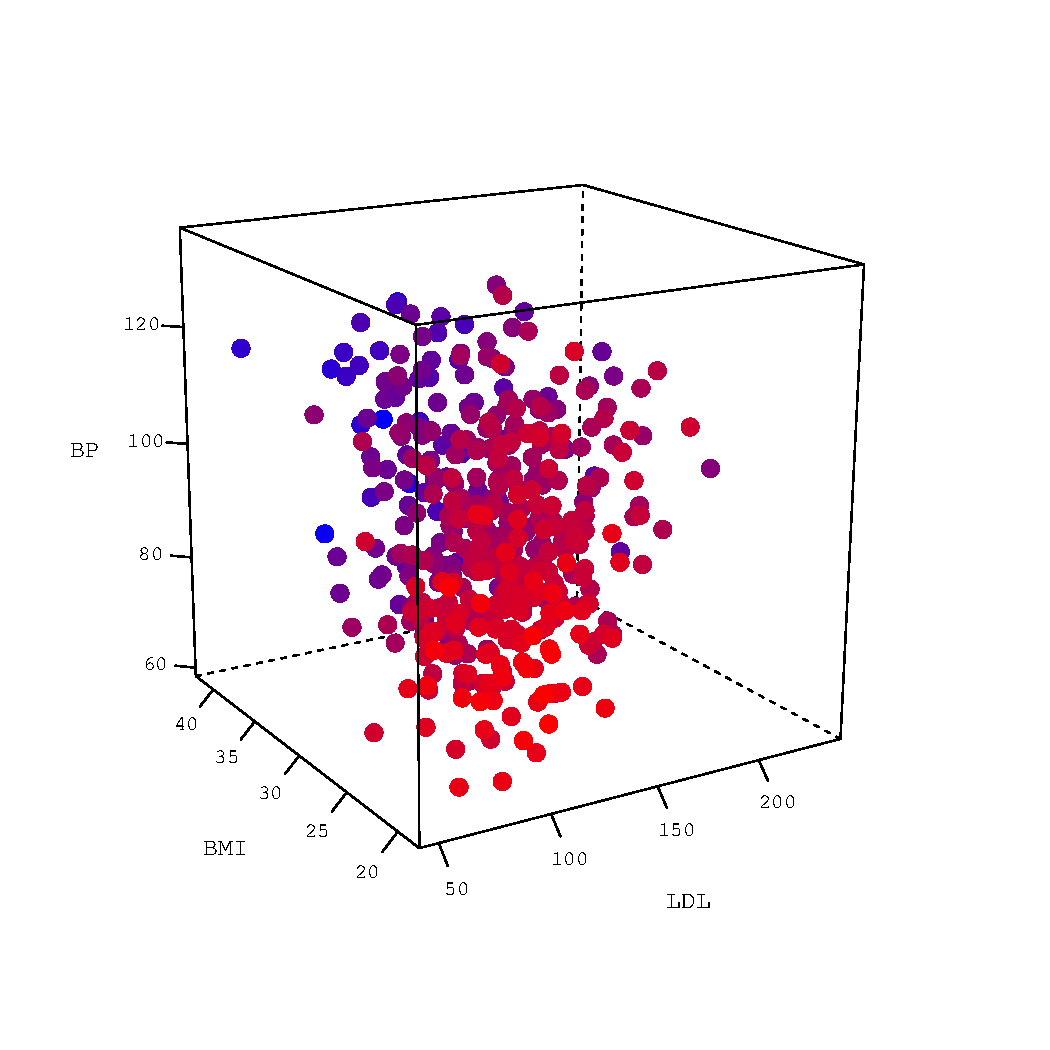
\includegraphics[width = 1.1\textwidth]{figures/3d_data_plot}
    \end{column}
    
    \begin{column}{0.1\textwidth}
      \begin{center}\Huge{$\rightarrow$}\end{center}
    \end{column}
    
    \begin{column}{0.45\textwidth}
      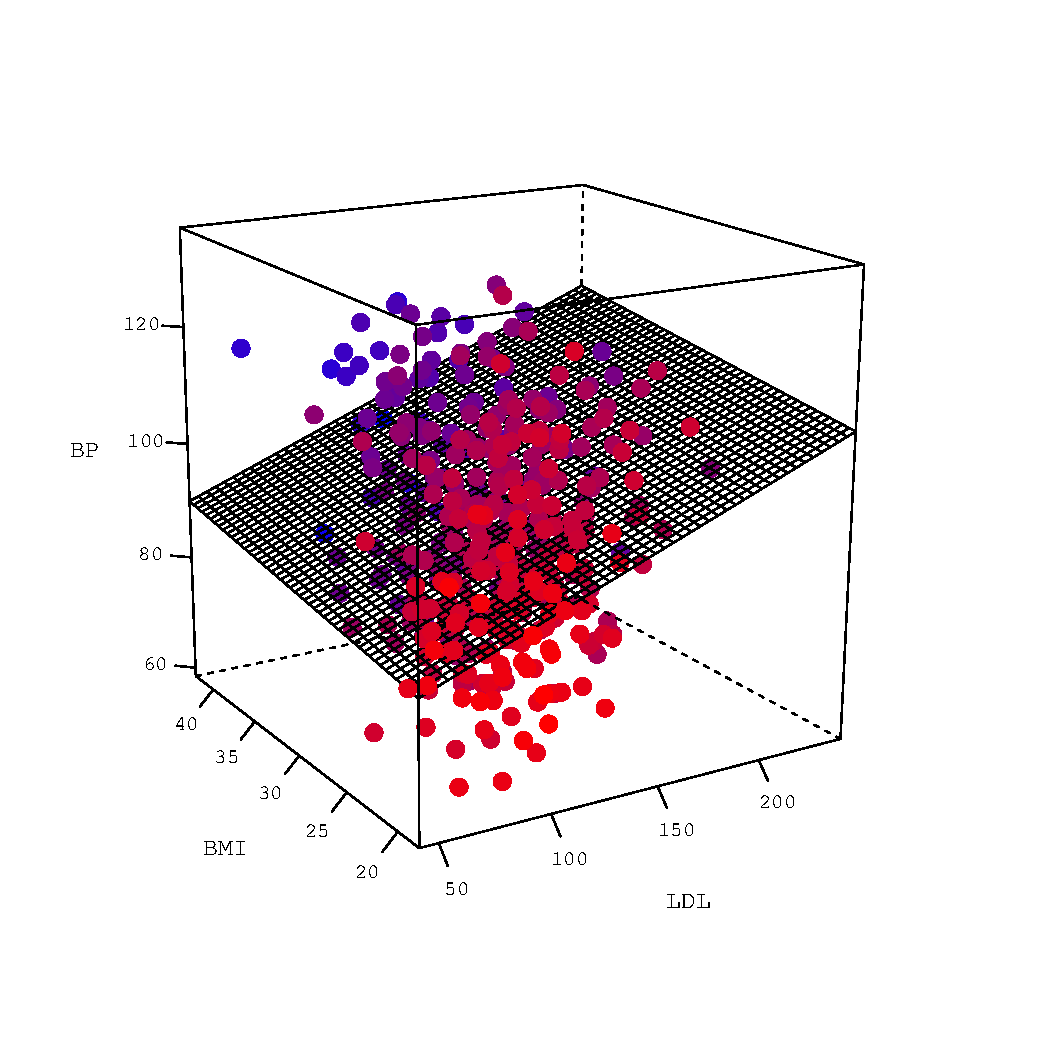
\includegraphics[width = 1.1\textwidth]{figures/response_surface_plot0}
    \end{column}
  \end{columns}
  
\end{frame}

%------------------------------------------------------------------------------%

\begin{frame}{Moderated Regression}
  
  The effect of $X$ on $Y$ varies \textbf{as a function} of $Z$.
  
  \begin{columns}
    \begin{column}{0.45\textwidth}
      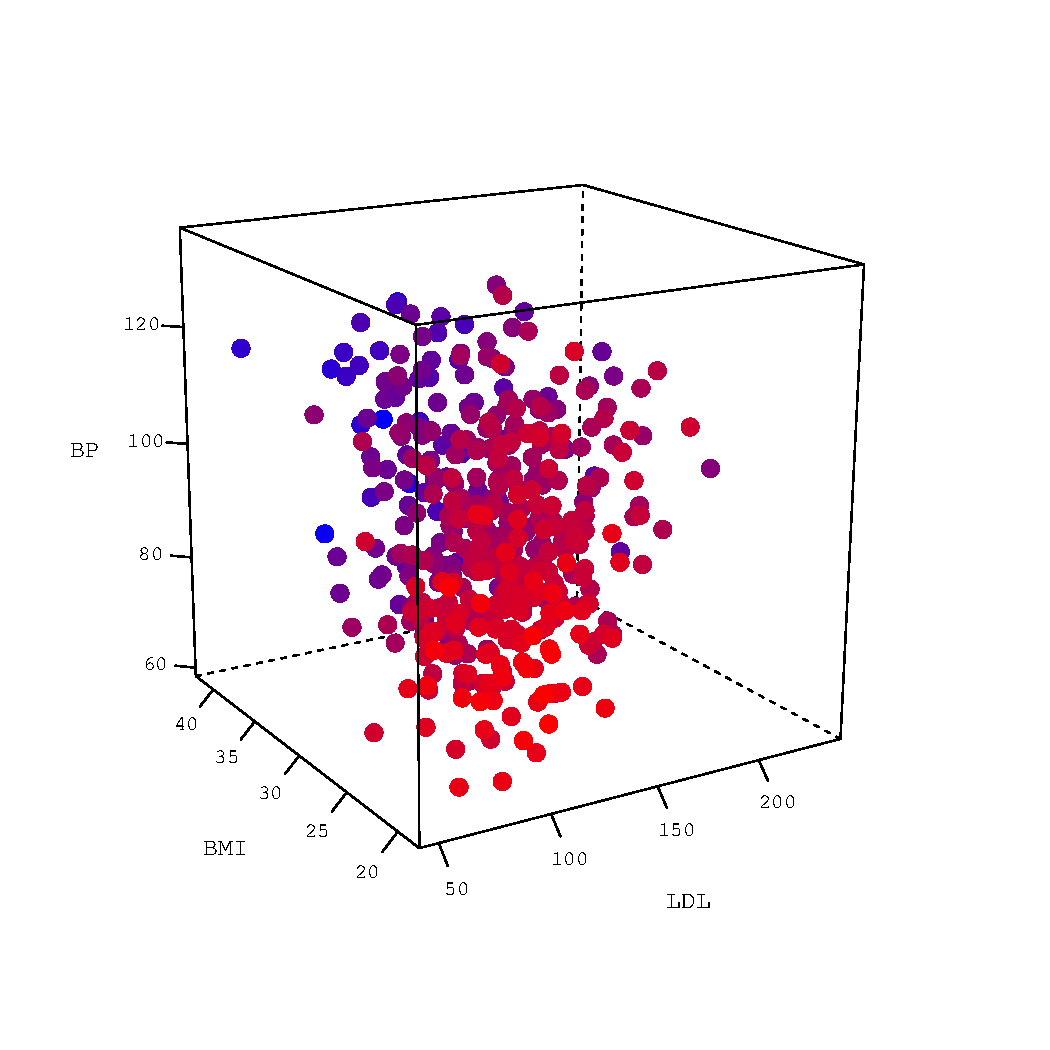
\includegraphics[width = 1.1\textwidth]{figures/3d_data_plot}
    \end{column}
    
    \begin{column}{0.1\textwidth}
      \begin{center}\Huge{$\rightarrow$}\end{center}
    \end{column}
    
    \begin{column}{0.45\textwidth}
      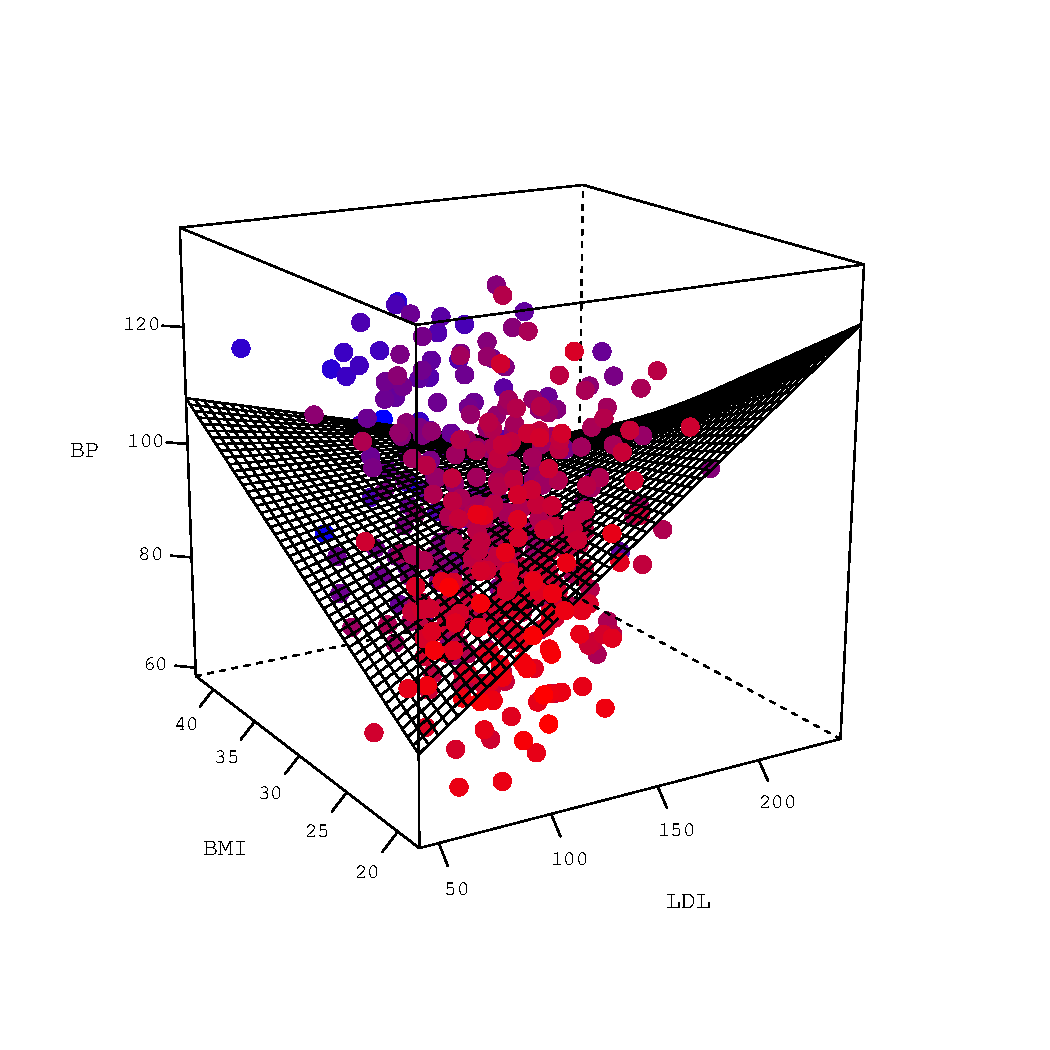
\includegraphics[width = 1.1\textwidth]{figures/response_surface_plot}
    \end{column}
  \end{columns}
  
\end{frame}

\watermarkon %-----------------------------------------------------------------%

\begin{frame}{Equations}
  
  The following derivation is adapted from \citet{hayes:2017}.
  \vb
  \begin{itemize}
  \item When testing moderation, we hypothesize that the effect of $X$ on $Y$ 
    varies as a function of $Z$.  
    \vb
  \item We can represent this concept with the following equation:
    \begin{align}
      Y = \beta_0 + f(Z)X + \beta_2Z + \varepsilon \label{fEq}
    \end{align}
    \vx{-8}
    \pause
  \item If we assume that $Z$ linearly (and deterministically) affects the 
    relationship between $X$ and $Y$, then we can take:
    \begin{align}
      f(Z) = \beta_1 + \beta_3Z \label{ssEq}
    \end{align}
  \end{itemize}
  
\end{frame}

%------------------------------------------------------------------------------%

\begin{frame}{Equations}
  
  \begin{itemize}
  \item Substituting Equation \ref{ssEq} into Equation \ref{fEq} leads to:
    \begin{align*}
      Y = \beta_0 + (\beta_1 + \beta_3Z)X + \beta_2Z + \varepsilon
    \end{align*}
    \pause
  \item Which, after distributing $X$ and reordering terms, becomes:
    \begin{align*}
      Y = \beta_0 + \beta_1X + \beta_2Z + \beta_3XZ + \varepsilon
    \end{align*}
  \end{itemize}
  
\end{frame}

%------------------------------------------------------------------------------%

\begin{frame}{Testing Moderation}
  Now, we have an estimable regression model that quantifies the linear 
  moderation we hypothesized.
  \vb
  \begin{center}\ovalbox{$Y = \beta_0 + \beta_1X + \beta_2Z + \beta_3XZ + 
      \varepsilon$}\end{center}
  \vc
  \begin{itemize}
  \item To test for significant moderation, we simply need to test the 
    significance of the interaction term, $XZ$.
    \begin{itemize}
    \item Check if $\hat{\beta}_3$ is significantly different from zero.
    \end{itemize}
  \end{itemize}
  
\end{frame}

%------------------------------------------------------------------------------%

\begin{frame}{Interpretation}
  
  Given the following equation:
  \begin{align*}
    Y = \hat{\beta}_0 + \hat{\beta}_1X + \hat{\beta}_2Z + \hat{\beta}_3XZ + 
    \hat{\varepsilon}
  \end{align*}
  \vx{-16}
  \begin{itemize}
  \item $\hat{\beta}_3$ quantifies the effect of $Z$ on the focal effect (the $X 
    \rightarrow Y$ effect).
    \vc
    \begin{itemize}
    \item For a unit change in $Z$, $\hat{\beta}_3$ is the expected change in
      the effect of $X$ on $Y$.
    \end{itemize}
    \vb
  \item $\hat{\beta}_1$ and $\hat{\beta}_2$ are \emph{conditional effects}.
    \vc
    \begin{itemize}
      \item Interpreted where the other predictor is zero.
        \vc
      \item For a unit change in $X$, $\hat{\beta}_1$ is the expected change in
        $Y$, when $Z = 0$.
        \vc
      \item For a unit change in $Z$, $\hat{\beta}_2$ is the expected change in
        $Y$, when $X = 0$.
    \end{itemize}
  \end{itemize}
  
\end{frame}

%------------------------------------------------------------------------------%
  
\begin{frame}{Example}
  
  Still looking at the \emph{diabetes} dataset.
  \va 
  \begin{itemize}
  \item We suspect that patients' BMIs are predictive of their average blood 
    pressure. 
    \va 
  \item We further suspect that this effect may be differentially expressed 
    depending on the patients' LDL levels.
  \end{itemize}
  
\end{frame}

\watermarkoff%-----------------------------------------------------------------%

\begin{frame}[fragile]{Example}



\begin{knitrout}\footnotesize
\definecolor{shadecolor}{rgb}{0.878, 0.918, 0.933}\color{fgcolor}\begin{kframe}
\begin{alltt}
\hlcom{## Focal Effect:}
\hlstd{out0} \hlkwb{<-} \hlkwd{lm}\hlstd{(bp} \hlopt{~} \hlstd{bmi,} \hlkwc{data} \hlstd{= dDat)}
\hlkwd{partSummary}\hlstd{(out0,} \hlopt{-}\hlkwd{c}\hlstd{(}\hlnum{1}\hlstd{,} \hlnum{2}\hlstd{))}
\end{alltt}
\begin{verbatim}
## Coefficients:
##             Estimate Std. Error t value Pr(>|t|)
## (Intercept)  61.9973     3.6659   16.91   <2e-16
## bmi           1.2379     0.1371    9.03   <2e-16
## 
## Residual standard error: 12.72 on 440 degrees of freedom
## Multiple R-squared:  0.1563,	Adjusted R-squared:  0.1544 
## F-statistic: 81.54 on 1 and 440 DF,  p-value: < 2.2e-16
\end{verbatim}
\end{kframe}
\end{knitrout}

\end{frame}

%------------------------------------------------------------------------------%

\begin{frame}[fragile]{Example}

\begin{knitrout}\footnotesize
\definecolor{shadecolor}{rgb}{0.878, 0.918, 0.933}\color{fgcolor}\begin{kframe}
\begin{alltt}
\hlcom{## Additive Model:}
\hlstd{out1} \hlkwb{<-} \hlkwd{lm}\hlstd{(bp} \hlopt{~} \hlstd{bmi} \hlopt{+} \hlstd{ldl,} \hlkwc{data} \hlstd{= dDat)}
\hlkwd{partSummary}\hlstd{(out1,} \hlopt{-}\hlkwd{c}\hlstd{(}\hlnum{1}\hlstd{,} \hlnum{2}\hlstd{))}
\end{alltt}
\begin{verbatim}
## Coefficients:
##             Estimate Std. Error t value Pr(>|t|)
## (Intercept) 59.26577    3.91281  15.147  < 2e-16
## bmi          1.16567    0.14156   8.235 2.08e-15
## ldl          0.04016    0.02056   1.953   0.0515
## 
## Residual standard error: 12.68 on 439 degrees of freedom
## Multiple R-squared:  0.1636,	Adjusted R-squared:  0.1598 
## F-statistic: 42.94 on 2 and 439 DF,  p-value: < 2.2e-16
\end{verbatim}
\end{kframe}
\end{knitrout}

\end{frame}

%------------------------------------------------------------------------------%

\begin{frame}[fragile]{Example}

\begin{knitrout}\footnotesize
\definecolor{shadecolor}{rgb}{0.878, 0.918, 0.933}\color{fgcolor}\begin{kframe}
\begin{alltt}
\hlcom{## Moderated Model:}
\hlstd{out2} \hlkwb{<-} \hlkwd{lm}\hlstd{(bp} \hlopt{~} \hlstd{bmi} \hlopt{*} \hlstd{ldl,} \hlkwc{data} \hlstd{= dDat)}
\hlkwd{partSummary}\hlstd{(out2,} \hlopt{-}\hlkwd{c}\hlstd{(}\hlnum{1}\hlstd{,} \hlnum{2}\hlstd{))}
\end{alltt}
\begin{verbatim}
## Coefficients:
##              Estimate Std. Error t value Pr(>|t|)
## (Intercept) 14.480616  14.291677   1.013 0.311514
## bmi          2.867825   0.541312   5.298 1.86e-07
## ldl          0.448771   0.127160   3.529 0.000461
## bmi:ldl     -0.015352   0.004716  -3.255 0.001221
## 
## Residual standard error: 12.54 on 438 degrees of freedom
## Multiple R-squared:  0.1834,	Adjusted R-squared:  0.1778 
## F-statistic: 32.78 on 3 and 438 DF,  p-value: < 2.2e-16
\end{verbatim}
\end{kframe}
\end{knitrout}

\end{frame}

%------------------------------------------------------------------------------%

\begin{frame}{Visualizing the Interaction}

  \begin{columns}
    \begin{column}{0.5\textwidth}
      We can get a better idea of the patterns of moderation by plotting the 
      focal effect at conditional values of the moderator.
    \end{column}
    
    \begin{column}{0.5\textwidth}
      
\begin{knitrout}\footnotesize
\definecolor{shadecolor}{rgb}{0.878, 0.918, 0.933}\color{fgcolor}

{\centering 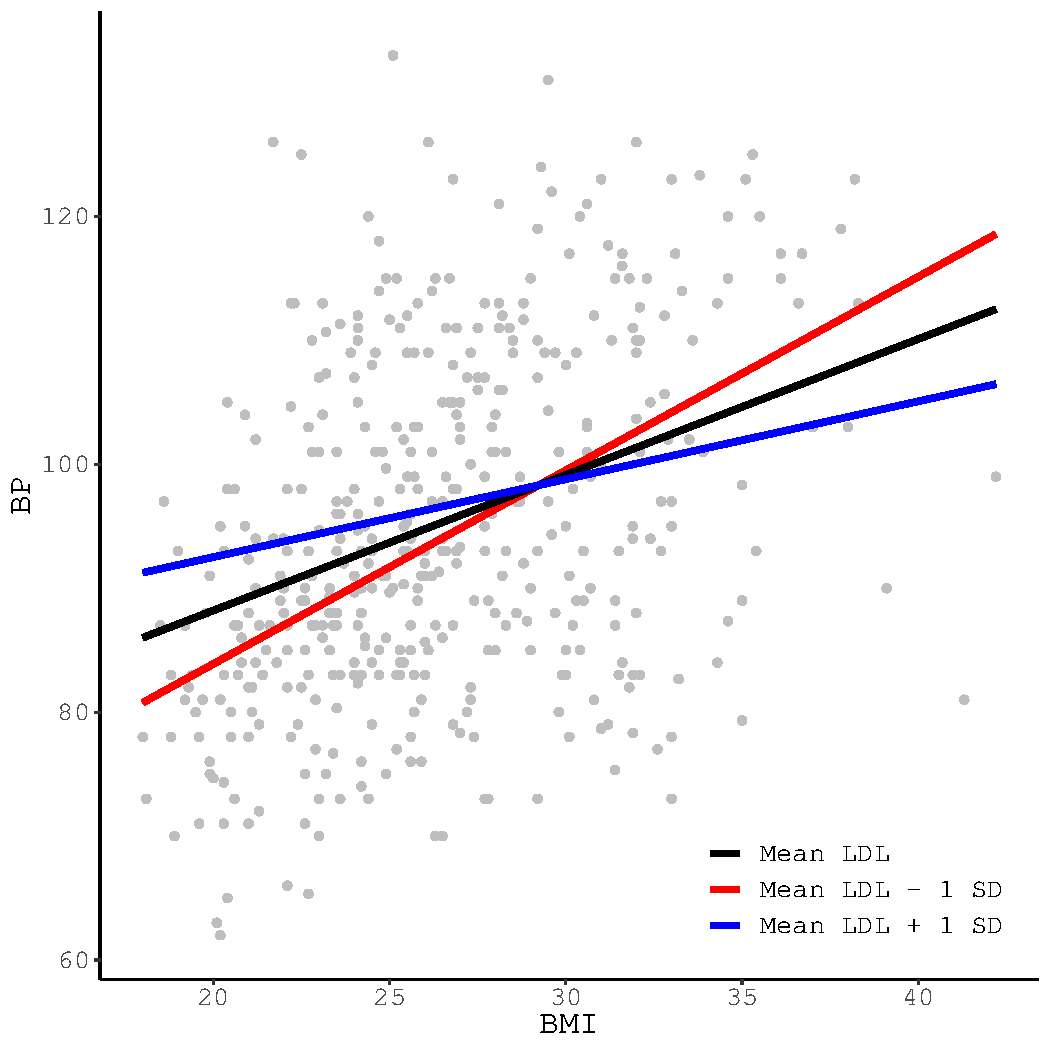
\includegraphics[width=\maxwidth]{figure/unnamed-chunk-5-1} 

}



\end{knitrout}

\end{column}
\end{columns}

\end{frame}

\watermarkon %-----------------------------------------------------------------%

\begin{frame}{Probing the Interaction}

  A significant estimate of $\beta_3$ tells us that the effect of $X$ on $Y$ 
  depends on the level of $Z$, but nothing more.
  \vb
  \begin{itemize}
  \item The plot on the previous slide gives a descriptive illustration of the 
    pattern, but does not support statistical inference.
    \vc
    \begin{itemize}
    \item The three conditional effects we plotted look different, but we cannot 
      say much about how they differ with only the plot and $\hat{\beta}_3$.
    \end{itemize}
    \vb
  \item This is the purpose of \emph{probing} the interaction.
    \vc
    \begin{itemize}
    \item Try to isolate areas of $Z$'s distribution in which $X \rightarrow Y$
      effect is significant and areas where it is not.
    \end{itemize}
  \end{itemize}
  
\end{frame}

%------------------------------------------------------------------------------%

\begin{frame}{Probing the Interaction}

  The most popular method of probing interactions is to do a so-called 
  \emph{simple slopes} analysis.
  \vc
  \begin{itemize}
  \item Pick-a-point approach
    \vc
  \item Spotlight analysis
  \end{itemize}
  \vb
  In simple slopes analysis, we test if the slopes of the conditional effects 
  plotted above are significantly different from zero.
  \vc
  \begin{itemize}
  \item To do so, we test the significance of \emph{simple slopes}.
  \end{itemize}
  
\end{frame}

%------------------------------------------------------------------------------%

\begin{frame}{Simple Slopes}

  Recall the derivation of our moderated equation:
  \begin{align*}
    Y = \beta_0 + \beta_1X + \beta_2Z + \beta_3XZ + \varepsilon
  \end{align*}
  We can reverse the process by factoring out $X$ and reordering terms:
  \begin{align*}
    Y = \beta_0 + (\beta_1 + \beta_3Z)X + \beta_2Z + \varepsilon
  \end{align*}
  Where $f(Z) = \beta_1 + \beta_3Z$ is the linear function that shows how the 
  relationship between $X$ and $Y$ changes as a function of $Z$.\\
  \vc
  \begin{center}
  \ovalbox{$f(Z)$ is the \emph{simple slope}.}
  \end{center}
  \begin{itemize}
  \item By plugging different values of $Z$ into $f(Z)$, we get the value of the 
    conditional effect of $X$ on $Y$ at the chosen level of $Z$.
  \end{itemize}

\end{frame}

%------------------------------------------------------------------------------%

\begin{frame}{Significance Testing of Simple Slopes}

  The values of $Z$ used to define the simple slopes are arbitrary.
  \vc
  \begin{itemize}
  \item The most common choice is: $\left\{ (\bar{Z} - SD_Z), \bar{Z},
    (\bar{Z} + SD_Z) \right\}$
    \vc
  \item You could also use interesting percentiles of $Z$'s distribution.
  \end{itemize}
  \vb
  The standard error of a simple slope is given by:
  \begin{align*}
    SE_{f(Z)} = \sqrt{SE_{\beta_1}^2 + 2Z \cdot \text{COV}(\beta_1, \beta_3) + 
      Z^2 SE_{\beta_3}^2}
  \end{align*}
  So, you can test the significance of a simple slope by constructing a Wald 
  statistic or confidence interval using $\hat{f}(Z)$ and $SE_{f(Z)}$:
  \begin{align*}
    t = \frac{\hat{f}(Z)}{SE_{f(Z)}},~~
    CI = \hat{f}(Z) \pm t_{crit} \times SE_{f(Z)}
  \end{align*}

\end{frame}

%------------------------------------------------------------------------------%

\begin{frame}{Interaction Probing}
  
  When probed the interaction with simple slopes analysis:
  \vb
  \begin{enumerate}
    \item Choose interesting values of the moderator, $Z$. \label{chooseZ}
      \vb
    \item Check the significance of the focal effect, $X \rightarrow Y$, at the 
      $Z$ values chosen in Step \ref{chooseZ}. \label{testSS}
      \vb
    \item Use the results from Step \ref{testSS} to get an idea of where in 
      $Z$'s distribution the focal effect is or is not significant.
  \end{enumerate}
  \va
  \pause
  We saw manual calculations for the the quantities needed, but there is a 
  simpler way:
  \vc
  \begin{itemize}
    \item \textsc{Centering}
  \end{itemize}
  
\end{frame}

%------------------------------------------------------------------------------%

\begin{frame}{Centering}
  
  Centering shifts the scale of a variable up or down by subtracting a constant 
  (e.g., the variable's mean) from each of its observations.
  \vc
  \begin{itemize}
  \item The most familiar form of center is \emph{mean centering}.
    \vc
  \item We can center on any value.
    \vc
    \begin{itemize}
    \item When probing interactions, we can center $Z$ on the interesting values
      we choose to define the simple slopes.
      \vc
    \item Due to the interpretation of conditional effects, running the model 
      with $Z$ centered on a specific value automatically provides a test of the 
      simple slope for that value of $Z$.
    \end{itemize}
  \end{itemize}
  
\end{frame}

%------------------------------------------------------------------------------%

\begin{frame}{Probing via Centering}
  
  Say we want to do a simple slopes analysis to test the conditional effect of 
  $X$ on $Y$ at three levels of $Z = \{Z_1, Z_2, Z_3\}$.
  \vb
  \begin{itemize}
  \item All we need to do is fit the following three models:
    \begin{align*}
      Y &= \beta_0 + \beta_1X + \beta_2(Z - Z_1) + \beta_3 X(Z - Z_1) + 
      \varepsilon\\[10pt]
      Y &= \beta_0 + \beta_1X + \beta_2(Z - Z_2) + \beta_3 X(Z - Z_2) + 
      \varepsilon\\[10pt]
      Y &= \beta_0 + \beta_1X + \beta_2(Z - Z_3) + \beta_3 X(Z - Z_3) + 
      \varepsilon
    \end{align*}
    \pause
    \vx{-12}
  \item The default output for $\hat{\beta}_1$ provides tests of the simple 
    slopes.
  \end{itemize}
  
\end{frame}

\watermarkoff %----------------------------------------------------------------%

\begin{frame}[fragile]{Example}

  Create transformed predictors by centering on critical values of the 
  moderator, $Z_{LDL}$.
\begin{knitrout}\footnotesize
\definecolor{shadecolor}{rgb}{0.878, 0.918, 0.933}\color{fgcolor}\begin{kframe}
\begin{alltt}
\hlstd{zMean}     \hlkwb{<-} \hlkwd{mean}\hlstd{(dDat}\hlopt{$}\hlstd{ldl)}
\hlstd{zSD}       \hlkwb{<-} \hlkwd{sd}\hlstd{(dDat}\hlopt{$}\hlstd{ldl)}
\hlstd{dDat}\hlopt{$}\hlstd{zCen} \hlkwb{<-} \hlstd{dDat}\hlopt{$}\hlstd{ldl} \hlopt{-} \hlstd{zMean}
\hlstd{dDat}\hlopt{$}\hlstd{zHi}  \hlkwb{<-} \hlstd{dDat}\hlopt{$}\hlstd{ldl} \hlopt{-} \hlstd{(zMean} \hlopt{+} \hlstd{zSD)}
\hlstd{dDat}\hlopt{$}\hlstd{zLo}  \hlkwb{<-} \hlstd{dDat}\hlopt{$}\hlstd{ldl} \hlopt{-} \hlstd{(zMean} \hlopt{-} \hlstd{zSD)}
\end{alltt}
\end{kframe}
\end{knitrout}

\end{frame}

%------------------------------------------------------------------------------%

\begin{frame}[fragile]{Example}

  Test the simple slope of $X_{BMI} \rightarrow Y_{BP}$ at 1 $SD$ below the mean 
  of $Z_{LDL}$.
\begin{knitrout}\footnotesize
\definecolor{shadecolor}{rgb}{0.878, 0.918, 0.933}\color{fgcolor}\begin{kframe}
\begin{alltt}
\hlstd{out2.1} \hlkwb{<-} \hlkwd{lm}\hlstd{(bp} \hlopt{~} \hlstd{bmi}\hlopt{*}\hlstd{zLo,} \hlkwc{data} \hlstd{= dDat)}
\hlkwd{partSummary}\hlstd{(out2.1,} \hlopt{-}\hlkwd{c}\hlstd{(}\hlnum{1}\hlstd{,} \hlnum{2}\hlstd{))}
\end{alltt}
\begin{verbatim}
## Coefficients:
##              Estimate Std. Error t value Pr(>|t|)
## (Intercept) 52.637886   4.764883  11.047  < 2e-16
## bmi          1.562525   0.185667   8.416 5.59e-16
## zLo          0.448771   0.127160   3.529 0.000461
## bmi:zLo     -0.015352   0.004716  -3.255 0.001221
## 
## Residual standard error: 12.54 on 438 degrees of freedom
## Multiple R-squared:  0.1834,	Adjusted R-squared:  0.1778 
## F-statistic: 32.78 on 3 and 438 DF,  p-value: < 2.2e-16
\end{verbatim}
\end{kframe}
\end{knitrout}
The estimated slope for \texttt{bmi}, $\hat{\beta}_1 = 
1.563$, is the simple slope.
 
\end{frame}

%------------------------------------------------------------------------------%

\begin{frame}[fragile]{Example}

  Test the simple slope of $X_{BMI} \rightarrow Y_{BP}$ at the mean of $Z_{LDL}$.
\begin{knitrout}\footnotesize
\definecolor{shadecolor}{rgb}{0.878, 0.918, 0.933}\color{fgcolor}\begin{kframe}
\begin{alltt}
\hlstd{out2.2} \hlkwb{<-} \hlkwd{lm}\hlstd{(bp} \hlopt{~} \hlstd{bmi}\hlopt{*}\hlstd{zCen,} \hlkwc{data} \hlstd{= dDat)}
\hlkwd{partSummary}\hlstd{(out2.2,} \hlopt{-}\hlkwd{c}\hlstd{(}\hlnum{1}\hlstd{,} \hlnum{2}\hlstd{))}
\end{alltt}
\begin{verbatim}
## Coefficients:
##              Estimate Std. Error t value Pr(>|t|)
## (Intercept) 66.286409   3.812480  17.387  < 2e-16
## bmi          1.095631   0.141679   7.733 7.27e-14
## zCen         0.448771   0.127160   3.529 0.000461
## bmi:zCen    -0.015352   0.004716  -3.255 0.001221
## 
## Residual standard error: 12.54 on 438 degrees of freedom
## Multiple R-squared:  0.1834,	Adjusted R-squared:  0.1778 
## F-statistic: 32.78 on 3 and 438 DF,  p-value: < 2.2e-16
\end{verbatim}
\end{kframe}
\end{knitrout}
The estimated slope for \texttt{bmi}, $\hat{\beta}_1 = 
1.096$, is the simple slope.
 
\end{frame}

%------------------------------------------------------------------------------%

\begin{frame}[fragile]{Example}
  
  Test the simple slope of $X_{BMI} \rightarrow Y_{BP}$ at 1 $SD$ above the mean 
  of $Z_{LDL}$.
\begin{knitrout}\footnotesize
\definecolor{shadecolor}{rgb}{0.878, 0.918, 0.933}\color{fgcolor}\begin{kframe}
\begin{alltt}
\hlstd{out2.3} \hlkwb{<-} \hlkwd{lm}\hlstd{(bp} \hlopt{~} \hlstd{bmi}\hlopt{*}\hlstd{zHi,} \hlkwc{data} \hlstd{= dDat)}
\hlkwd{partSummary}\hlstd{(out2.3,} \hlopt{-}\hlkwd{c}\hlstd{(}\hlnum{1}\hlstd{,} \hlnum{2}\hlstd{))}
\end{alltt}
\begin{verbatim}
## Coefficients:
##              Estimate Std. Error t value Pr(>|t|)
## (Intercept) 79.934933   6.023132  13.271  < 2e-16
## bmi          0.628736   0.216369   2.906 0.003848
## zHi          0.448771   0.127160   3.529 0.000461
## bmi:zHi     -0.015352   0.004716  -3.255 0.001221
## 
## Residual standard error: 12.54 on 438 degrees of freedom
## Multiple R-squared:  0.1834,	Adjusted R-squared:  0.1778 
## F-statistic: 32.78 on 3 and 438 DF,  p-value: < 2.2e-16
\end{verbatim}
\end{kframe}
\end{knitrout}
The estimated slope for \texttt{bmi}, $\hat{\beta}_1 = 
0.629$, is the simple slope.
 
\end{frame}

%------------------------------------------------------------------------------%

\captionsetup{labelformat=empty}
\begin{frame}{Compare Approaches}
  
  The manual and the centering approaches give identical answers, barring 
  rounding errors: 
  \vb
% latex table generated in R 4.0.2 by xtable 1.8-4 package
% Thu Oct  1 10:12:34 2020
\begin{table}[ht]
\centering
\begin{tabular}{rccc}
  \toprule
 & Z Low & Z Center & Z High \\ 
  \midrule
Manual & 1.562525 & 1.095631 & 0.628736 \\ 
  Centering & 1.562525 & 1.095631 & 0.628736 \\ 
   \bottomrule
\end{tabular}
\caption{Simple Slopes} 
\end{table}


\vx{-6}

% latex table generated in R 4.0.2 by xtable 1.8-4 package
% Thu Oct  1 10:12:34 2020
\begin{table}[ht]
\centering
\begin{tabular}{rccc}
  \toprule
 & Z Low & Z Center & Z High \\ 
  \midrule
Manual & 0.185667 & 0.141679 & 0.216369 \\ 
  Centering & 0.185667 & 0.141679 & 0.216369 \\ 
   \bottomrule
\end{tabular}
\caption{Standard Errors} 
\end{table}


\end{frame}
\captionsetup{labelformat=default}

\watermarkon %-----------------------------------------------------------------%

\begin{frame}{Alternative Probing Strategies}
  
  Simple slopes analysis is nice due to its simplicity and ease of
  interpretation, but the $Z$ values we choose are totally arbitrary.
  \vc
  \begin{itemize}
  \item We may be missing important nuances that occur in areas of $Z$'s 
    distribution that we \emph{did not} pick.
  \end{itemize}
  \vb
  \pause
  The \emph{Johnson-Neyman} technique is an alternative approach that removes 
  the arbitrary selection of conditional $Z$ values.
  \vc
  \begin{itemize}
  \item Johnson-Neyman finds the \emph{region of significance} wherein the 
    conditional effect of $X$ on $Y$ is statistically significant.
    \vc
  \item Johnson-Neyman inverts the logic of simple slopes analysis to find what 
    cut-points on the moderator correspond to a critical $t$ value for the 
    conditional effect.
  \end{itemize}
  
\end{frame}

%------------------------------------------------------------------------------%

\begin{frame}{Johnson-Neyman Technique}
  
  With simple slopes analysis, we:
  \vb
  \begin{enumerate}
    \item Choose a conditional value of $Z$, say $Z_1$.
      \vb
    \item Calculate the simple slope, $\hat{f}(Z_1)$, and standard error, 
      $SE_{f(Z_1)}$, associated with $Z_1$.
      \vb
    \item Test $\hat{f}(Z_1)$ for significance via a simple Wald-type test:
      \begin{align}
        \hat{t} = \frac{\hat{f}(Z_1)}{SE_{f(Z_1)}} \label{waldEq}
      \end{align}
  \end{enumerate}

\end{frame}

%------------------------------------------------------------------------------%

\begin{frame}{Johnson-Neyman Technique}
  
  With Johnson-Neyman, we:
  \vb
  \begin{enumerate}
  \item Choose an $\alpha$ level for our test.
    \begin{itemize}
    \item Use $\{\alpha, df\}$ to define a critical $t$-value
      \begin{itemize}
      \item E.g., $\alpha = 0.05$ and $df = 438$ $\Rightarrow$ $t_{crit} = 1.97$
      \end{itemize}
    \end{itemize}
    \vb
  \item Replace $\hat{t}$ in Equation \ref{waldEq} with $t_{crit}$ and re-arrange 
    into the following quadratic form:
    \begin{align}
      t_{crit}^2 SE_{f(Z)}^2 - \hat{f}^2(Z) = 0 \label{quadEq}
    \end{align}
  \item Solve Equation \ref{quadEq} to find the two values of $Z$ (i.e., the 
    roots) that produce critical $t$ statistics for the simple slope.
  \end{enumerate}
  
\end{frame}

%------------------------------------------------------------------------------%

\begin{frame}{Deriving Equation \ref{quadEq}}
  
  Recall the definitions of $\hat{f}(Z)$ and $SE_{f(Z)}$:
  \begin{align*}
    \hat{f}(Z) &= \hat{\beta}_1 + \hat{\beta}_3Z,\\[10pt]
    SE_{f(Z)} &= \sqrt{SE_{\beta_1}^2 + 2Z \cdot \text{COV}(\beta_1, \beta_3) + Z^2 SE_{\beta_3}^2}.
  \end{align*}
  So, our starting point is:
  \begin{align}
    t_{crit} = \frac{\hat{\beta}_1 + \hat{\beta}_3Z}{\sqrt{SE_{\beta_1}^2 + 2Z \cdot \text{COV}(\beta_1, \beta_3) + Z^2 SE_{\beta_3}^2}}. \label{tEq0}
  \end{align}
  
\end{frame}

%------------------------------------------------------------------------------%

\begin{frame}{Deriving Equation \ref{quadEq}}
  
  Square both sides of Equation \ref{tEq0} to get:
  \begin{align}
    t_{crit}^2 = \frac{\hat{\beta}_1^2 + 2\hat{\beta}_1\hat{\beta}_3Z + \hat{\beta}_3^2Z^2}{SE_{\beta_1}^2 + 2Z \cdot \text{COV}(\beta_1, \beta_3) + Z^2 SE_{\beta_3}^2}. \label{t2Eq}
    \end{align}
  Lastly, move all terms in Equation \ref{t2Eq} to the left-hand side and 
  simplify to get the final quadratic form:
  \begin{align*}
    \left( t_{crit}^2 SE_{\beta_3}^2 - \hat{\beta}_3^2 \right) Z^2 +
    \left( 2t_{crit}^2 \text{COV}(\beta_1, \beta_3) - 2 \hat{\beta}_1 \hat{\beta}_3 \right) Z +
    \left( t_{crit}^2 SE_{\beta_1}^2 - \hat{\beta}_1^2 \right) = 0.
  \end{align*}
  
\end{frame}

%------------------------------------------------------------------------------%

\begin{frame}{Solving Equation \ref{quadEq}}
  
  Given our final quadratic equation:
  \begin{align*}
    \left( t_{crit}^2 SE_{\beta_3}^2 - \hat{\beta}_3^2 \right) Z^2 +
    \left( 2t_{crit}^2 \text{COV}(\beta_1, \beta_3) - 2 \hat{\beta}_1 \hat{\beta}_3 \right) Z +
    \left( t_{crit}^2 SE_{\beta_1}^2 - \hat{\beta}_1^2 \right) = 0,
  \end{align*}
  we find our solutions by taking:
  \begin{align*}
    a &= t_{crit}^2 SE_{\beta_3}^2 - \hat{\beta}_3^2,\\[8pt]
    b &= 2t_{crit}^2 \text{COV}(\beta_1, \beta_3) - 2 \hat{\beta}_1 \hat{\beta}_3,\\[8pt]
    c &= t_{crit}^2 SE_{\beta_1}^2 - \hat{\beta}_1^2,
  \end{align*}
  and applying the quadratic formula:
  \begin{align*}
    x = \frac{-b \pm \sqrt{b^2 - 4ac}}{2a}.
  \end{align*}
  
\end{frame}
    
\watermarkoff %----------------------------------------------------------------%

\begin{frame}[fragile, allowframebreaks]{Example}
  
\begin{knitrout}\footnotesize
\definecolor{shadecolor}{rgb}{0.878, 0.918, 0.933}\color{fgcolor}\begin{kframe}
\begin{alltt}
\hlcom{## Estimate model:}
\hlstd{out} \hlkwb{<-} \hlkwd{lm}\hlstd{(bp} \hlopt{~} \hlstd{bmi}\hlopt{*}\hlstd{ldl,} \hlkwc{data} \hlstd{= dDat)}

\hlcom{## Get (squared) critical value of t:}
\hlstd{t2} \hlkwb{<-} \hlkwd{qt}\hlstd{(}\hlnum{0.975}\hlstd{,} \hlkwc{df} \hlstd{= out}\hlopt{$}\hlstd{df.residual)}\hlopt{^}\hlnum{2}

\hlcom{## Extract pertinent elements from the asymptotic }
\hlcom{## covariance matrix:}
\hlstd{aCov} \hlkwb{<-} \hlkwd{vcov}\hlstd{(out)}
\hlstd{v1}   \hlkwb{<-} \hlkwd{diag}\hlstd{(aCov)[}\hlstr{"bmi"}\hlstd{]}
\hlstd{v3}   \hlkwb{<-} \hlkwd{diag}\hlstd{(aCov)[}\hlstr{"bmi:ldl"}\hlstd{]}
\hlstd{cv}   \hlkwb{<-} \hlstd{aCov[}\hlstr{"bmi"}\hlstd{,} \hlstr{"bmi:ldl"}\hlstd{]}

\hlcom{## Extract pertinent slope coefficients:}
\hlstd{b1} \hlkwb{<-} \hlkwd{coef}\hlstd{(out)[}\hlstr{"bmi"}\hlstd{]}
\hlstd{b3} \hlkwb{<-} \hlkwd{coef}\hlstd{(out)[}\hlstr{"bmi:ldl"}\hlstd{]}
\end{alltt}
\end{kframe}
\end{knitrout}

\pagebreak

\begin{knitrout}\footnotesize
\definecolor{shadecolor}{rgb}{0.878, 0.918, 0.933}\color{fgcolor}\begin{kframe}
\begin{alltt}
\hlcom{## Compute coefficients of the quadratic equation:}
\hlstd{a} \hlkwb{<-} \hlkwd{as.numeric}\hlstd{(t2} \hlopt{*} \hlstd{v3} \hlopt{-} \hlstd{b3}\hlopt{^}\hlnum{2}\hlstd{)}
\hlstd{b} \hlkwb{<-} \hlkwd{as.numeric}\hlstd{(}\hlnum{2} \hlopt{*} \hlstd{t2} \hlopt{*} \hlstd{cv} \hlopt{-} \hlnum{2} \hlopt{*} \hlstd{b1} \hlopt{*} \hlstd{b3)}
\hlstd{c} \hlkwb{<-} \hlkwd{as.numeric}\hlstd{(t2} \hlopt{*} \hlstd{v1} \hlopt{-} \hlstd{b1}\hlopt{^}\hlnum{2}\hlstd{)}

\hlcom{## Compute roots:}
\hlstd{myRoots} \hlkwb{<-} \hlkwd{c}\hlstd{(}
\hlstd{(}\hlopt{-}\hlstd{b} \hlopt{+} \hlkwd{sqrt}\hlstd{(b}\hlopt{^}\hlnum{2} \hlopt{-} \hlnum{4} \hlopt{*} \hlstd{a} \hlopt{*} \hlstd{c))} \hlopt{/} \hlstd{(}\hlnum{2} \hlopt{*} \hlstd{a),}
\hlstd{(}\hlopt{-}\hlstd{b} \hlopt{-} \hlkwd{sqrt}\hlstd{(b}\hlopt{^}\hlnum{2} \hlopt{-} \hlnum{4} \hlopt{*} \hlstd{a} \hlopt{*} \hlstd{c))} \hlopt{/} \hlstd{(}\hlnum{2} \hlopt{*} \hlstd{a)}
\hlstd{)}

\hlstd{myRoots}
\end{alltt}
\begin{verbatim}
## [1] 154.7983 305.9235
\end{verbatim}
\end{kframe}
\end{knitrout}

\end{frame}

\watermarkon %-----------------------------------------------------------------%

\begin{frame}{Interpreting Johnson-Neyman}
  
  The roots produced by the Johnson-Neyman technique delineate the
  \emph{region of significance}.  
  \vb
  \begin{itemize}
  \item The conditional effect of $X$ on $Y$ is either significant everywhere 
    inside or outside of the interval defined by these two points.  
    \vb
  \item If only one of the points falls within the observed range of $Z$, ignore 
    the other point. 
    \vc
    \begin{itemize}
    \item In this case, the region of significance is either everywhere above or 
      everywhere below the legal root.
    \end{itemize}
    \vb
  \item If neither of the roots fall within the observed range of $Z$, then you 
    are in one of two cases:
    \vc
    \begin{enumerate}
    \item The focal effect is significant across the entire range of $Z$. 
      \vc
    \item The focal effect is not significant anywhere within the range of $Z$.
    \end{enumerate}
  \end{itemize}
  
\end{frame}

\watermarkoff %----------------------------------------------------------------%

\begin{frame}[fragile]{Interpreting Johnson-Neyman}
  
\begin{knitrout}\footnotesize
\definecolor{shadecolor}{rgb}{0.878, 0.918, 0.933}\color{fgcolor}\begin{kframe}
\begin{alltt}
\hlstd{myRoots}
\end{alltt}
\begin{verbatim}
## [1] 154.7983 305.9235
\end{verbatim}
\begin{alltt}
\hlkwd{partSummary}\hlstd{(out2,} \hlopt{-}\hlkwd{c}\hlstd{(}\hlnum{1}\hlstd{,} \hlnum{2}\hlstd{))}
\end{alltt}
\begin{verbatim}
## Coefficients:
##              Estimate Std. Error t value Pr(>|t|)
## (Intercept) 14.480616  14.291677   1.013 0.311514
## bmi          2.867825   0.541312   5.298 1.86e-07
## ldl          0.448771   0.127160   3.529 0.000461
## bmi:ldl     -0.015352   0.004716  -3.255 0.001221
## 
## Residual standard error: 12.54 on 438 degrees of freedom
## Multiple R-squared:  0.1834,	Adjusted R-squared:  0.1778 
## F-statistic: 32.78 on 3 and 438 DF,  p-value: < 2.2e-16
\end{verbatim}
\end{kframe}
\end{knitrout}

\end{frame}

\watermarkon %-----------------------------------------------------------------%

\begin{frame}{Perspectives on Simple Slopes}
  
  Recall the formula for a simple slope:
  \begin{align*}
    f(Z) = \beta_1 + \beta_3Z
  \end{align*}
  \vc We can think about working with $f(Z)$ in, at least, two different ways:
  \vb
  \begin{enumerate}
  \item Treat $f(Z)$ as a weight for $X$ that we can use to evaluate the effect 
    of $X$ on $Y$ at different (discrete) levels of $Z$.
    \vb
  \item Consider how $f(Z)$, itself, changes as $Z$ (continuously) changes.  
  \end{enumerate}
  \vb
  The first option gives rise to simple slopes analysis while the second 
  embodies the spirit of Johnson-Neyman.
  
\end{frame}

%------------------------------------------------------------------------------%

\begin{frame}{Confidence Bands}
  
  A natural quantity to consider is a confidence interval for $\hat{f}(Z)$:
  \begin{align*}
    CI = \hat{f}(Z) \pm t_{crit} \times SE_{f(Z)}
  \end{align*}
  \vx{-16}
  \begin{itemize}
  \item We can easily computed such intervals for the interesting values of $Z$ 
    that we chose for the simple slopes analysis.
  \end{itemize}
  \pause
  \vb
  When doing Johnson-Neyman, we can compute the pointwise values of the $CI$ for
  the entire range of $Z$.  
  \vb
  \begin{itemize}
  \item Interpolating between these pointwise CIs produces \emph{confidence 
    bands} for $\hat{f}(Z)$.
    \vc
    \begin{itemize}
    \item With these confidence bands, we can immediately check any value of $Z$ 
      for a significant simple slope.
    \end{itemize}
  \end{itemize}
  
\end{frame}

\watermarkoff %----------------------------------------------------------------%
  
\begin{frame}[fragile, allowframebreaks]{Example}
  
  Implementing the Johnson-Neyman technique by hand is a pain, but we can easily 
  do so by using the \textbf{rockchalk} package in \textsf{R}.\\ 
  
  \vb
  
\begin{knitrout}\footnotesize
\definecolor{shadecolor}{rgb}{0.878, 0.918, 0.933}\color{fgcolor}\begin{kframe}
\begin{alltt}
\hlkwd{library}\hlstd{(rockchalk)}

\hlcom{## First we need to create a 'plotSlopes' object:}
\hlstd{plotOut} \hlkwb{<-} \hlkwd{plotSlopes}\hlstd{(}\hlkwc{model}      \hlstd{= out2,}
                      \hlkwc{plotx}      \hlstd{=} \hlstr{"bmi"}\hlstd{,}
                      \hlkwc{modx}       \hlstd{=} \hlstr{"ldl"}\hlstd{,}
                      \hlkwc{plotPoints} \hlstd{=} \hlnum{FALSE}\hlstd{)}
\end{alltt}
\end{kframe}

{\centering 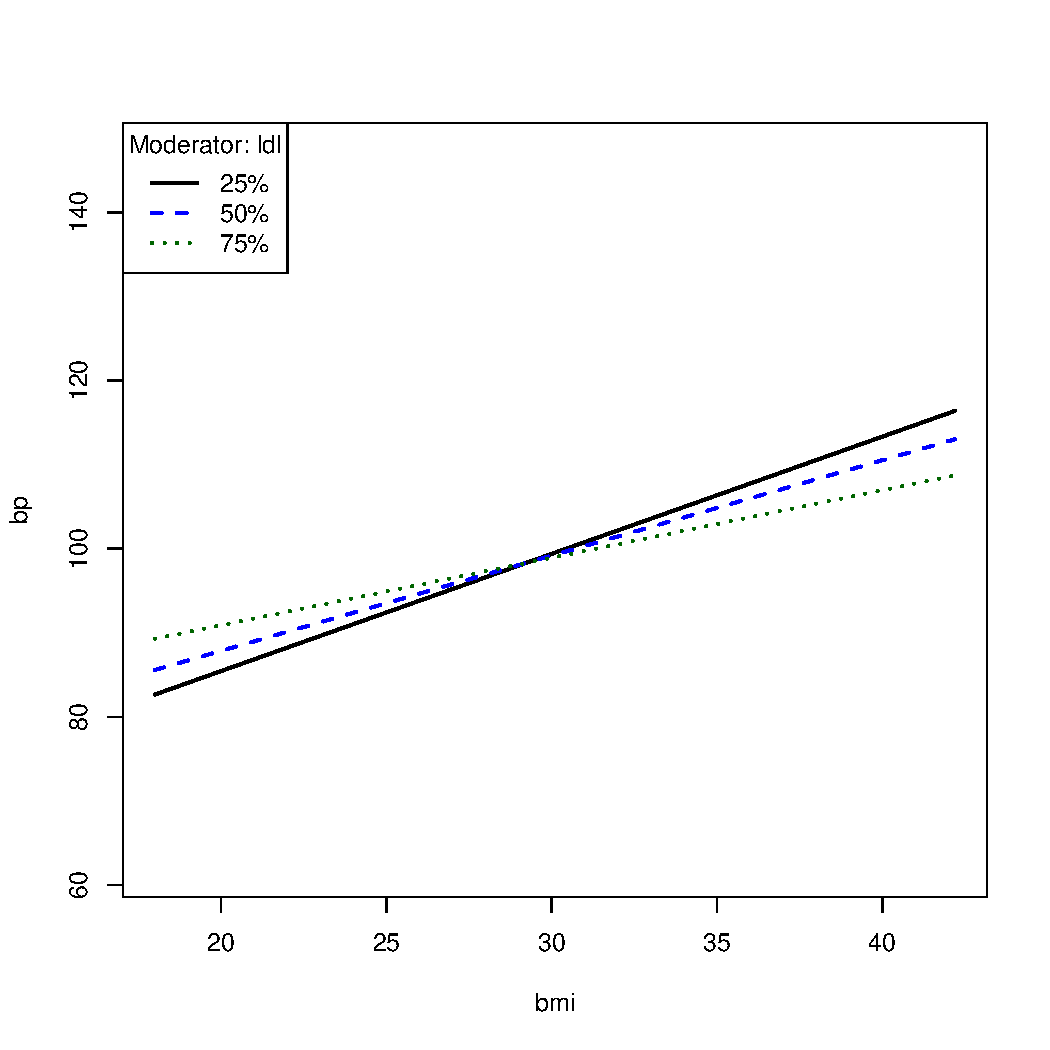
\includegraphics[width=0.65\linewidth]{figure/unnamed-chunk-15-1} 

}



\end{knitrout}

\end{frame}

%------------------------------------------------------------------------------%

\begin{frame}[fragile]{Example}

  We conduct the Johnson-Neyman test by using the \texttt{testSlopes} function 
  to modify the ``plotSlopes'' object:
  
\begin{knitrout}\footnotesize
\definecolor{shadecolor}{rgb}{0.878, 0.918, 0.933}\color{fgcolor}\begin{kframe}
\begin{alltt}
\hlcom{## Implement the J-N test:}
\hlkwd{wrap}\hlstd{(testOut} \hlkwb{<-} \hlkwd{testSlopes}\hlstd{(plotOut))}
\end{alltt}
\begin{verbatim}
## Values of ldl OUTSIDE this interval:
##       lo       hi 
## 154.7983 305.9235 
## cause the slope of (b1 + b2*ldl)bmi to be statistically 
## significant
\end{verbatim}
\begin{alltt}
\hlcom{## Extract the significance boundaries:}
\hlstd{testOut}\hlopt{$}\hlstd{jn}\hlopt{$}\hlstd{roots}
\end{alltt}
\begin{verbatim}
##       lo       hi 
## 154.7983 305.9235
\end{verbatim}
\end{kframe}
\end{knitrout}

\end{frame}

%------------------------------------------------------------------------------%
  
\begin{frame}[fragile]{Example}

  \begin{columns}
    \begin{column}{0.35\textwidth}
      
      Finally, we can plot the result:
      
\begin{knitrout}\footnotesize
\definecolor{shadecolor}{rgb}{0.878, 0.918, 0.933}\color{fgcolor}\begin{kframe}
\begin{alltt}
\hlkwd{plot}\hlstd{(testOut)}
\end{alltt}
\end{kframe}
\end{knitrout}

\end{column}
\begin{column}{0.65\textwidth}
  


{\centering 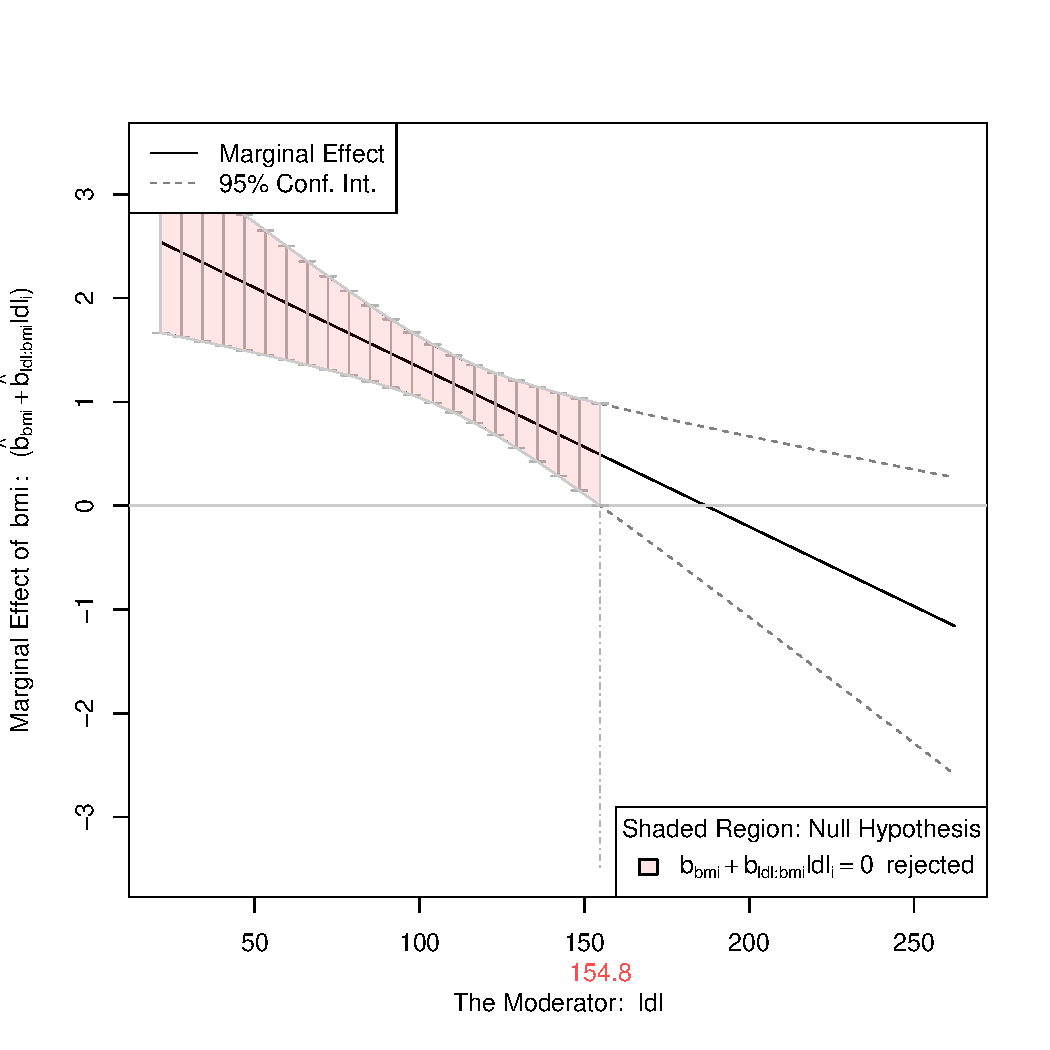
\includegraphics[width=\maxwidth]{figure/unnamed-chunk-18-1} 

}




\end{column}
\end{columns}

\end{frame}

%------------------------------------------------------------------------------%

\captionsetup{labelformat = empty}
\begin{frame}{Compare Implementations}
  
  As expected, we get the same answers from our manual solution and from the 
  \textbf{rockchalk} implementation.
  
% latex table generated in R 4.0.2 by xtable 1.8-4 package
% Thu Oct  1 10:12:35 2020
\begin{table}[ht]
\centering
\begin{tabular}{rrr}
  \toprule
 & Low & High \\ 
  \midrule
Manual & 154.80 & 305.92 \\ 
  Rockchalk & 154.80 & 305.92 \\ 
   \bottomrule
\end{tabular}
\caption{Johnson-Neyman Roots} 
\end{table}


\end{frame}
\captionsetup{labelformat = default}

\watermarkon %-----------------------------------------------------------------%

\begin{frame}{Categorical Moderators}
  
  Categorical moderators encode \emph{group-specific} effects.
  \vb
  \begin{itemize}
  \item E.g., if we include \emph{sex} as a moderator, we are modeling separate
    focal effects for males and females.
  \end{itemize}
  \va 
  Given a set of codes representing our moderator, we specify the
  interactions as before:
  \begin{align*}
    Y_{total} &= \beta_0 + \beta_1 X_{inten} + \beta_2 Z_{male} + 
    \beta_3 X_{inten}Z_{male} + \varepsilon\\\\
    Y_{total} &= \beta_0 + \beta_1 X_{inten} + \beta_2 Z_{lo} + \beta_3 Z_{mid} + 
    \beta_4 Z_{hi}\\ 
    &+ \beta_5 X_{inten}Z_{lo} + \beta_6 X_{inten}Z_{mid} + \beta_7 X_{inten}Z_{hi} + 
    \varepsilon
  \end{align*}
  
\end{frame}

\watermarkoff %----------------------------------------------------------------%

\begin{frame}[fragile]{Example}
  
\begin{knitrout}\footnotesize
\definecolor{shadecolor}{rgb}{0.878, 0.918, 0.933}\color{fgcolor}\begin{kframe}
\begin{alltt}
\hlcom{## Load data:}
\hlstd{socSup} \hlkwb{<-} \hlkwd{readRDS}\hlstd{(}\hlkwd{paste0}\hlstd{(dataDir,} \hlstr{"social_support.rds"}\hlstd{))}

\hlcom{## Focal effect:}
\hlstd{out3} \hlkwb{<-} \hlkwd{lm}\hlstd{(bdi} \hlopt{~} \hlstd{tanSat,} \hlkwc{data} \hlstd{= socSup)}
\hlkwd{partSummary}\hlstd{(out3,} \hlopt{-}\hlkwd{c}\hlstd{(}\hlnum{1}\hlstd{,} \hlnum{2}\hlstd{))}
\end{alltt}
\begin{verbatim}
## Coefficients:
##             Estimate Std. Error t value Pr(>|t|)
## (Intercept)  24.4089     5.3502   4.562 1.54e-05
## tanSat       -0.8100     0.3124  -2.593   0.0111
## 
## Residual standard error: 9.278 on 93 degrees of freedom
## Multiple R-squared:  0.06742,	Adjusted R-squared:  0.05739 
## F-statistic: 6.723 on 1 and 93 DF,  p-value: 0.01105
\end{verbatim}
\end{kframe}
\end{knitrout}

\end{frame}

%------------------------------------------------------------------------------%

\begin{frame}[fragile]{Example}

\begin{knitrout}\footnotesize
\definecolor{shadecolor}{rgb}{0.878, 0.918, 0.933}\color{fgcolor}\begin{kframe}
\begin{alltt}
\hlcom{## Estimate the interaction:}
\hlstd{out4} \hlkwb{<-} \hlkwd{lm}\hlstd{(bdi} \hlopt{~} \hlstd{tanSat} \hlopt{*} \hlstd{sex,} \hlkwc{data} \hlstd{= socSup)}
\hlkwd{partSummary}\hlstd{(out4,} \hlopt{-}\hlkwd{c}\hlstd{(}\hlnum{1}\hlstd{,} \hlnum{2}\hlstd{))}
\end{alltt}
\begin{verbatim}
## Coefficients:
##                Estimate Std. Error t value Pr(>|t|)
## (Intercept)     20.8478     6.2114   3.356  0.00115
## tanSat          -0.5772     0.3614  -1.597  0.11372
## sexmale         14.3667    12.2054   1.177  0.24223
## tanSat:sexmale  -0.9482     0.7177  -1.321  0.18978
## 
## Residual standard error: 9.267 on 91 degrees of freedom
## Multiple R-squared:  0.08955,	Adjusted R-squared:  0.05954 
## F-statistic: 2.984 on 3 and 91 DF,  p-value: 0.03537
\end{verbatim}
\end{kframe}
\end{knitrout}

\end{frame}

%------------------------------------------------------------------------------%

\begin{frame}[fragile]{Example}

  On the last slide, the estimated slope for \texttt{tanSat}, $\hat{\beta}_1 = 
  -0.577$, is the simple slope for females.
  \vc
  \begin{itemize}
  \item To estimate the simple slope for males, we simply change the reference 
    group of the \texttt{sex} factor and re-estimate the model.
  \end{itemize}
  
\begin{knitrout}\footnotesize
\definecolor{shadecolor}{rgb}{0.878, 0.918, 0.933}\color{fgcolor}\begin{kframe}
\begin{alltt}
\hlcom{## Test the 'male' simple slope by changing reference group:}
\hlstd{socSup}\hlopt{$}\hlstd{sex2} \hlkwb{<-} \hlkwd{relevel}\hlstd{(socSup}\hlopt{$}\hlstd{sex,} \hlkwc{ref} \hlstd{=} \hlstr{"male"}\hlstd{)}

\hlcom{## Re-estimate the interaction:}
\hlstd{out5} \hlkwb{<-} \hlkwd{lm}\hlstd{(bdi} \hlopt{~} \hlstd{tanSat} \hlopt{*} \hlstd{sex2,} \hlkwc{data} \hlstd{= socSup)}
\end{alltt}
\end{kframe}
\end{knitrout}

\end{frame}

%------------------------------------------------------------------------------%

\begin{frame}[fragile]{Example}

\begin{knitrout}\footnotesize
\definecolor{shadecolor}{rgb}{0.878, 0.918, 0.933}\color{fgcolor}\begin{kframe}
\begin{alltt}
\hlkwd{partSummary}\hlstd{(out5,} \hlopt{-}\hlkwd{c}\hlstd{(}\hlnum{1}\hlstd{,} \hlnum{2}\hlstd{))}
\end{alltt}
\begin{verbatim}
## Coefficients:
##                   Estimate Std. Error t value Pr(>|t|)
## (Intercept)        35.2146    10.5067   3.352  0.00117
## tanSat             -1.5254     0.6201  -2.460  0.01579
## sex2female        -14.3667    12.2054  -1.177  0.24223
## tanSat:sex2female   0.9482     0.7177   1.321  0.18978
## 
## Residual standard error: 9.267 on 91 degrees of freedom
## Multiple R-squared:  0.08955,	Adjusted R-squared:  0.05954 
## F-statistic: 2.984 on 3 and 91 DF,  p-value: 0.03537
\end{verbatim}
\end{kframe}
\end{knitrout}

The estimated slope for \texttt{tanSat}, $\hat{\beta}_1 = 
-1.525$, is now the simple slope for males.

\end{frame}

%------------------------------------------------------------------------------%

\begin{frame}[fragile]{Visualizing Categorical Moderation}

  \begin{columns}
    \begin{column}{0.5\textwidth}
      {\scriptsize
        \vx{-12}
        \begin{align*}
          \hat{Y}_{BDI} &= 20.85 
            -0.58 X_{tsat} + 
              14.37 Z_{male}\\ 
                &-0.95 
                  X_{tsat} Z_{male}
        \end{align*}
        \vx{-12}
      }
\begin{knitrout}\footnotesize
\definecolor{shadecolor}{rgb}{0.878, 0.918, 0.933}\color{fgcolor}

{\centering 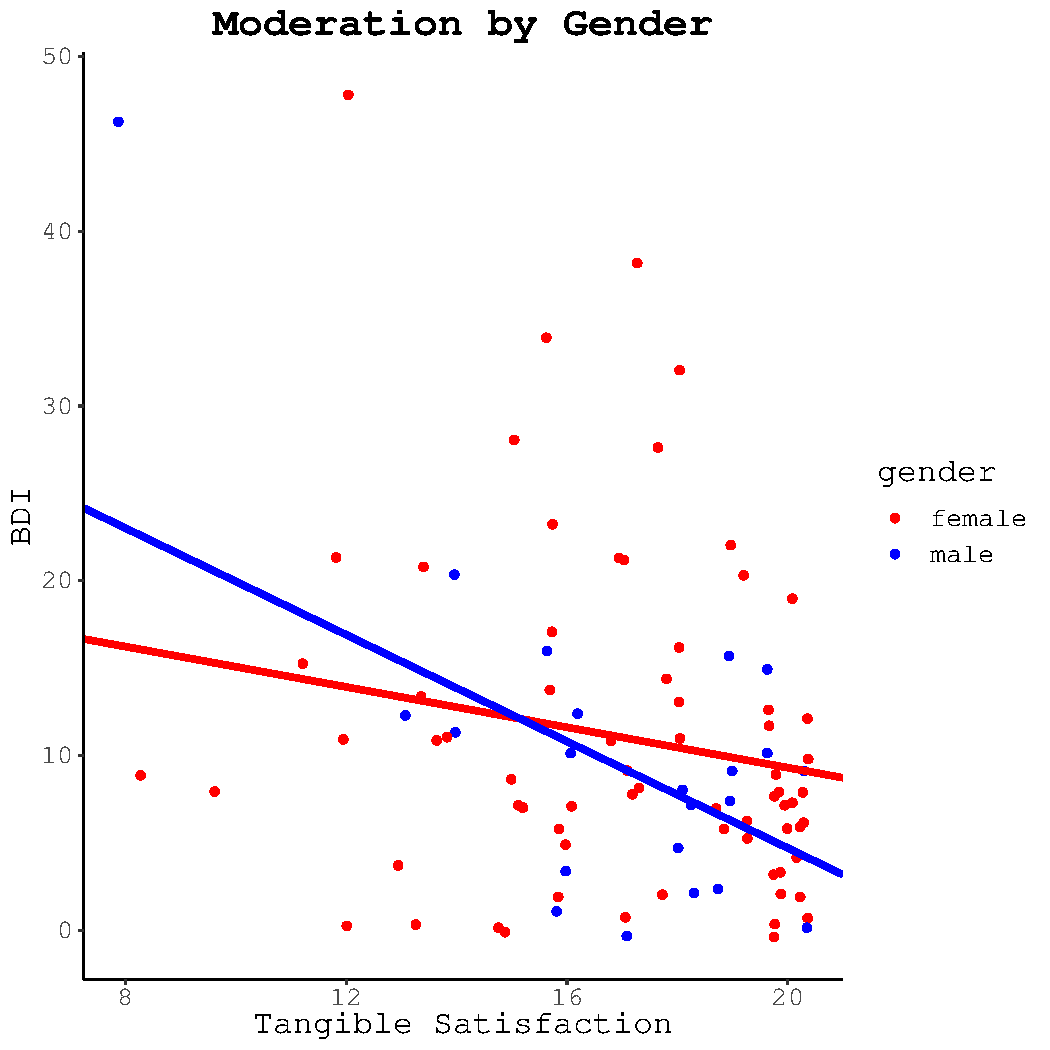
\includegraphics[width=\maxwidth]{figure/unnamed-chunk-24-1} 

}



\end{knitrout}

\end{column}

\begin{column}{0.5\textwidth}
  {\scriptsize
    \begin{align*}
      \hat{Y}_{BDI} = 28.10  
      -1.00 X_{tsat}  
      -1.05 Z_{male}
    \end{align*}
    \vx{-6}
  }
\begin{knitrout}\footnotesize
\definecolor{shadecolor}{rgb}{0.878, 0.918, 0.933}\color{fgcolor}

{\centering 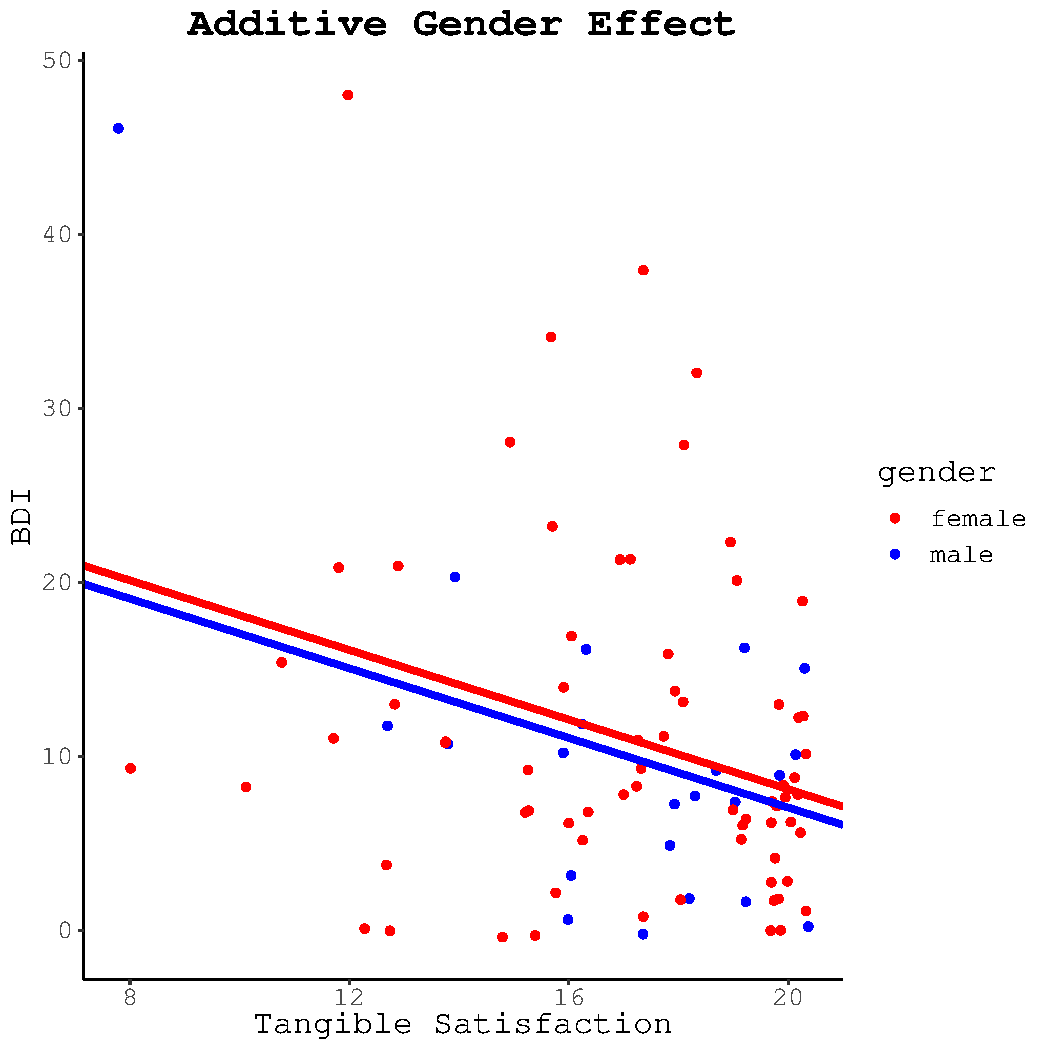
\includegraphics[width=\maxwidth]{figure/unnamed-chunk-25-1} 

}



\end{knitrout}

\end{column}
\end{columns}

\end{frame}

\watermarkon %-----------------------------------------------------------------%

\begin{frame}{}
  
  \begin{center}
    \Huge{\textsc{Polynomial Regression}}
  \end{center}
  
\end{frame}

%------------------------------------------------------------------------------%

\begin{frame}{Polynomial Regression}
  
  Polynomial regression simply incorporates powered transformations of the
  predictors into the model.
  \vb
  \begin{itemize}
  \item Polynomial terms (i.e., power terms) model curvature in the
    relationships.
  \end{itemize}
  \va
  We can think about polynomial terms as interactions between a predictor and 
  itself.
  \vb
  \begin{itemize}
  \item Many of the rules that apply to interactions transfer directly to
    polynomials.
  \end{itemize}
  
\end{frame}

\watermarkoff %----------------------------------------------------------------%

\begin{frame}{Polynomial Visualization}
  
  \begin{columns}
    \begin{column}{0.5\textwidth}
      We may hypothesize a curvilinear relationship between $X$ and $Y$.
    \end{column}
    
    \begin{column}{0.5\textwidth}
      
\begin{knitrout}\footnotesize
\definecolor{shadecolor}{rgb}{0.878, 0.918, 0.933}\color{fgcolor}

{\centering 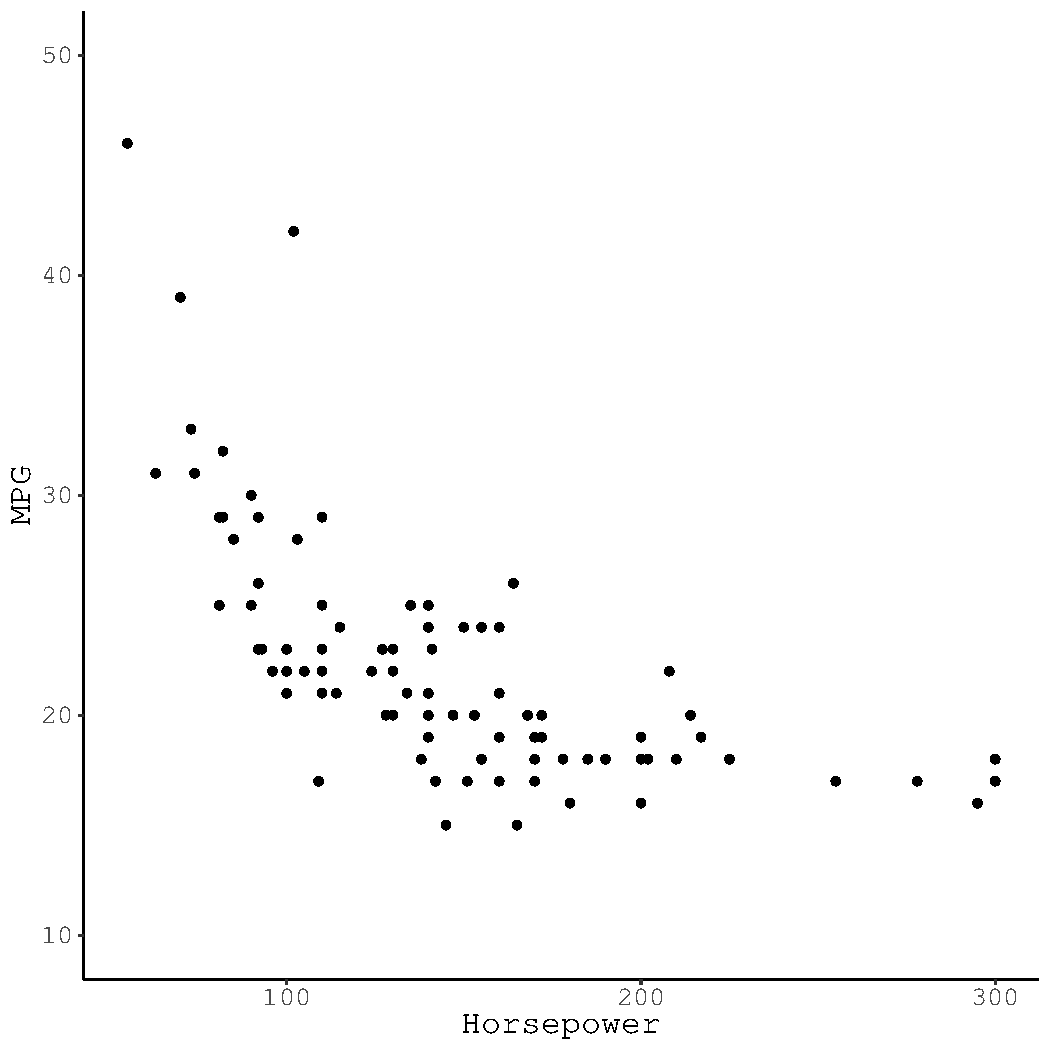
\includegraphics[width=\maxwidth]{figure/unnamed-chunk-26-1} 

}



\end{knitrout}

\end{column}
\end{columns}

\end{frame}

%------------------------------------------------------------------------------%

\begin{frame}{Polynomial Visualization}
  
  \begin{columns}
    \begin{column}{0.5\textwidth}
      Polynomials are one way to model curvilinear relationships.
      \vb
      \begin{itemize}  
      \item {\color{blue}$\hat{Y}_{mpg} = \hat{\beta}_0 + \hat{\beta}_1 X_{hp}$}
        \vb
      \item {\color{red}$\hat{Y}_{mpg} = \hat{\beta}_0 + \hat{\beta}_1 X_{hp} + 
        \hat{\beta}_2 X_{hp}^2$}
        \vb
      \item {\color{violet}$\hat{Y}_{mpg} = \hat{\beta}_0 + \hat{\beta}_1 X_{hp} + 
        \hat{\beta}_2 X_{hp}^2 + \hat{\beta}_3 X_{hp}^3$}
      \end{itemize}
    \end{column}
    
    \begin{column}{0.5\textwidth}
      
\begin{knitrout}\footnotesize
\definecolor{shadecolor}{rgb}{0.878, 0.918, 0.933}\color{fgcolor}

{\centering 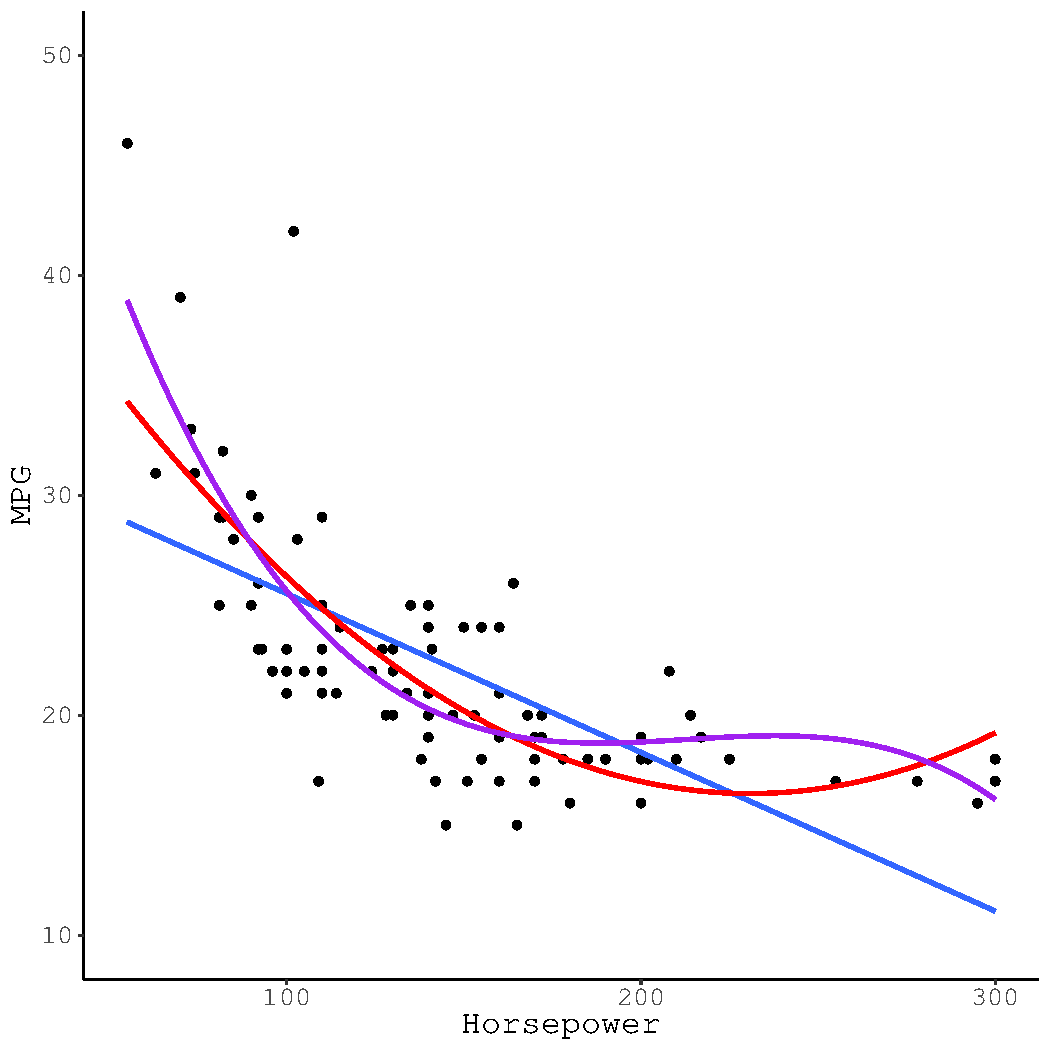
\includegraphics[width=\maxwidth]{figure/unnamed-chunk-27-1} 

}



\end{knitrout}

\end{column}
\end{columns}

\end{frame}

%------------------------------------------------------------------------------%

\begin{frame}[fragile, allowframebreaks]{Example}

\begin{knitrout}\footnotesize
\definecolor{shadecolor}{rgb}{0.878, 0.918, 0.933}\color{fgcolor}\begin{kframe}
\begin{alltt}
\hlcom{## Attach the data:}
\hlkwd{data}\hlstd{(Cars93)}

\hlcom{## Fit the linear model:}
\hlstd{out6} \hlkwb{<-} \hlkwd{lm}\hlstd{(MPG.city} \hlopt{~} \hlstd{Horsepower,} \hlkwc{data} \hlstd{= Cars93)}

\hlcom{## Fit the quadratic model:}
\hlstd{out7} \hlkwb{<-} \hlkwd{lm}\hlstd{(MPG.city} \hlopt{~} \hlstd{Horsepower} \hlopt{+} \hlkwd{I}\hlstd{(Horsepower}\hlopt{^}\hlnum{2}\hlstd{),}
           \hlkwc{data} \hlstd{= Cars93)}
\end{alltt}
\end{kframe}
\end{knitrout}

\pagebreak

\begin{knitrout}\footnotesize
\definecolor{shadecolor}{rgb}{0.878, 0.918, 0.933}\color{fgcolor}\begin{kframe}
\begin{alltt}
\hlkwd{partSummary}\hlstd{(out6,} \hlopt{-}\hlkwd{c}\hlstd{(}\hlnum{1}\hlstd{,} \hlnum{2}\hlstd{))}
\end{alltt}
\begin{verbatim}
## Coefficients:
##              Estimate Std. Error t value Pr(>|t|)
## (Intercept) 32.746279   1.273229  25.719  < 2e-16
## Horsepower  -0.072174   0.008323  -8.671 1.54e-13
## 
## Residual standard error: 4.181 on 91 degrees of freedom
## Multiple R-squared:  0.4524,	Adjusted R-squared:  0.4464 
## F-statistic: 75.19 on 1 and 91 DF,  p-value: 1.537e-13
\end{verbatim}
\end{kframe}
\end{knitrout}
  
\begin{itemize}
\item For each unit increase in horsepower, the expected change in fuel economy 
  is $\hat{\beta}_1 = -0.0722$ units.
\end{itemize}

\end{frame}

%------------------------------------------------------------------------------%

\begin{frame}[fragile]{Example}

\begin{knitrout}\footnotesize
\definecolor{shadecolor}{rgb}{0.878, 0.918, 0.933}\color{fgcolor}\begin{kframe}
\begin{alltt}
\hlkwd{partSummary}\hlstd{(out7,} \hlopt{-}\hlkwd{c}\hlstd{(}\hlnum{1}\hlstd{,} \hlnum{2}\hlstd{))}
\end{alltt}
\begin{verbatim}
## Coefficients:
##                   Estimate Std. Error t value Pr(>|t|)
## (Intercept)      4.714e+01  2.544e+00  18.528  < 2e-16
## Horsepower      -2.660e-01  3.186e-02  -8.350 7.71e-13
## I(Horsepower^2)  5.762e-04  9.239e-05   6.237 1.42e-08
## 
## Residual standard error: 3.513 on 90 degrees of freedom
## Multiple R-squared:  0.6177,	Adjusted R-squared:  0.6092 
## F-statistic:  72.7 on 2 and 90 DF,  p-value: < 2.2e-16
\end{verbatim}
\end{kframe}
\end{knitrout}
\vx{-6}
\begin{itemize}
\item Extrapolating from powerless cars, each unit increase in 
  horsepower, is expected to change fuel economy by $\hat{\beta}_1 = 
  -0.266$ units.
  \vc
\item For a unit increase in horsepower, the effect of horsepower on fuel 
  economy is expected to increase by $\hat{\beta}_2 = 
  \ensuremath{5.76\times 10^{-4}}$ units.
\end{itemize}

\end{frame}

%------------------------------------------------------------------------------%

\begin{frame}[fragile, allowframebreaks]{Example}

Does adding the quadratic term explain a significantly larger proportion of
variability?
\begin{knitrout}\footnotesize
\definecolor{shadecolor}{rgb}{0.878, 0.918, 0.933}\color{fgcolor}\begin{kframe}
\begin{alltt}
\hlkwd{anova}\hlstd{(out6, out7)}
\end{alltt}
\begin{verbatim}
## Analysis of Variance Table
## 
## Model 1: MPG.city ~ Horsepower
## Model 2: MPG.city ~ Horsepower + I(Horsepower^2)
##   Res.Df    RSS Df Sum of Sq      F    Pr(>F)    
## 1     91 1591.0                                  
## 2     90 1110.9  1    480.11 38.897 1.424e-08 ***
## ---
## Signif. codes:  
## 0 '***' 0.001 '**' 0.01 '*' 0.05 '.' 0.1 ' ' 1
\end{verbatim}
\end{kframe}
\end{knitrout}

\pagebreak

Does adding the quadratic term reduce prediction error?
\begin{knitrout}\footnotesize
\definecolor{shadecolor}{rgb}{0.878, 0.918, 0.933}\color{fgcolor}\begin{kframe}
\begin{alltt}
\hlkwd{cv.lm}\hlstd{(}\hlkwc{data}   \hlstd{= Cars93,}
      \hlkwc{models} \hlstd{=} \hlkwd{c}\hlstd{(}\hlkwd{formula}\hlstd{(out6),} \hlkwd{formula}\hlstd{(out7)),}
      \hlkwc{K}      \hlstd{=} \hlnum{5}\hlstd{,}
      \hlkwc{names}  \hlstd{=} \hlkwd{c}\hlstd{(}\hlstr{"line"}\hlstd{,} \hlstr{"quad"}\hlstd{)}
      \hlstd{)}
\end{alltt}
\begin{verbatim}
##     line     quad 
## 17.93996 13.03084
\end{verbatim}
\end{kframe}
\end{knitrout}

\end{frame}

%------------------------------------------------------------------------------%

\begin{frame}{Effects of Centering}
  
  \begin{columns}
    \begin{column}{0.5\textwidth}
      
\begin{knitrout}\footnotesize
\definecolor{shadecolor}{rgb}{0.878, 0.918, 0.933}\color{fgcolor}

{\centering 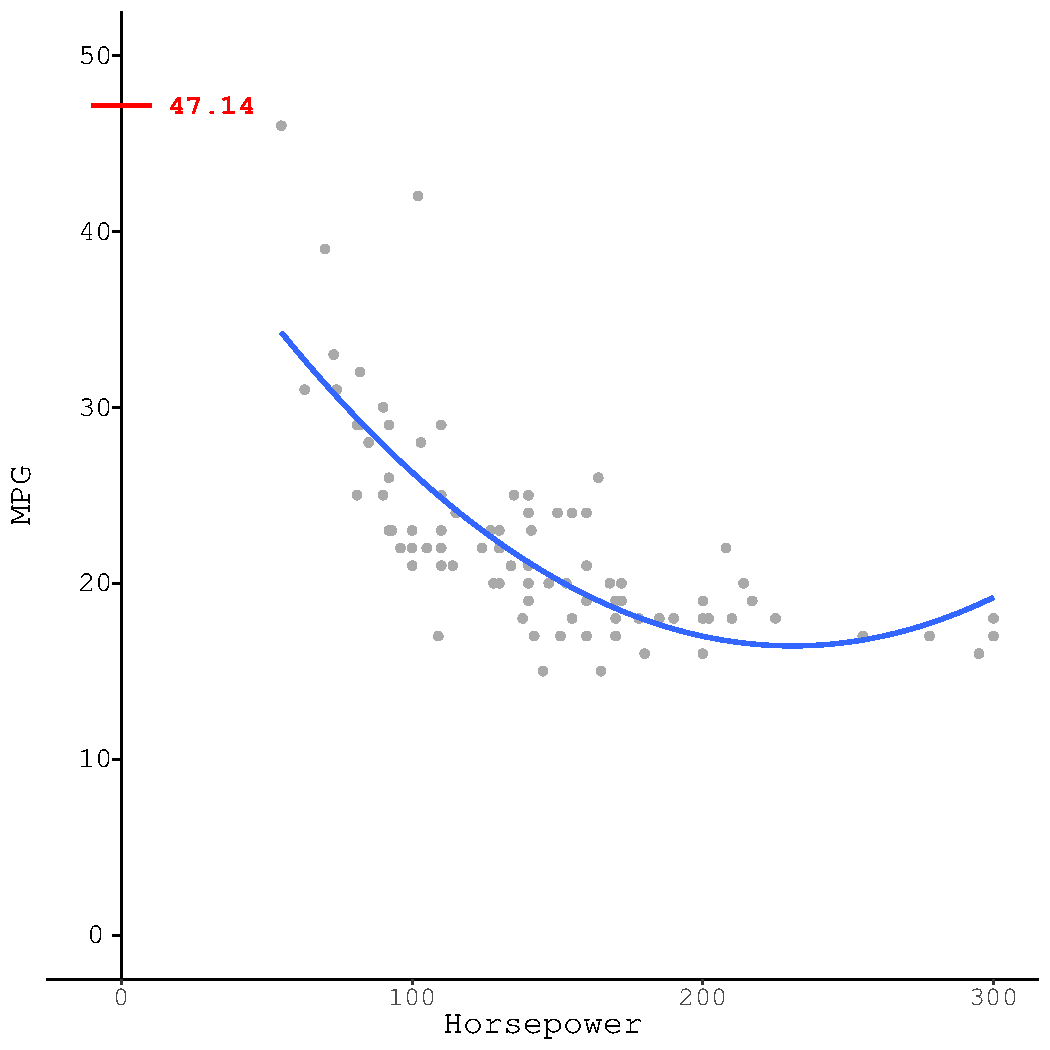
\includegraphics[width=\maxwidth]{figure/unnamed-chunk-33-1} 

}



\end{knitrout}

\end{column}
    
    \begin{column}{0.5\textwidth}
      
\begin{knitrout}\footnotesize
\definecolor{shadecolor}{rgb}{0.878, 0.918, 0.933}\color{fgcolor}

{\centering 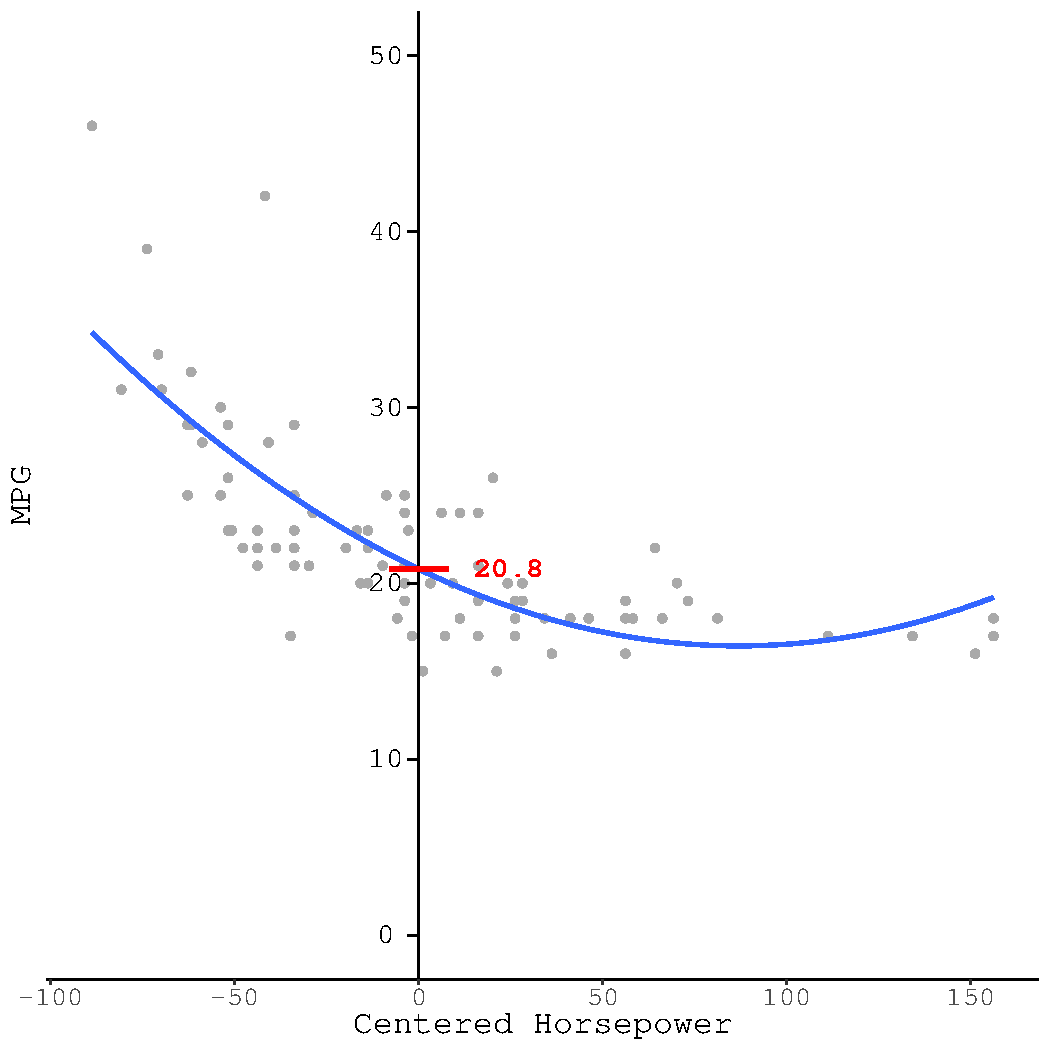
\includegraphics[width=\maxwidth]{figure/unnamed-chunk-34-1} 

}



\end{knitrout}

\end{column}
\end{columns}

\end{frame}

%------------------------------------------------------------------------------%
    
\begin{frame}{Effects of Centering}
  
  \begin{columns}
    \begin{column}{0.5\textwidth}
      
\begin{knitrout}\footnotesize
\definecolor{shadecolor}{rgb}{0.878, 0.918, 0.933}\color{fgcolor}

{\centering 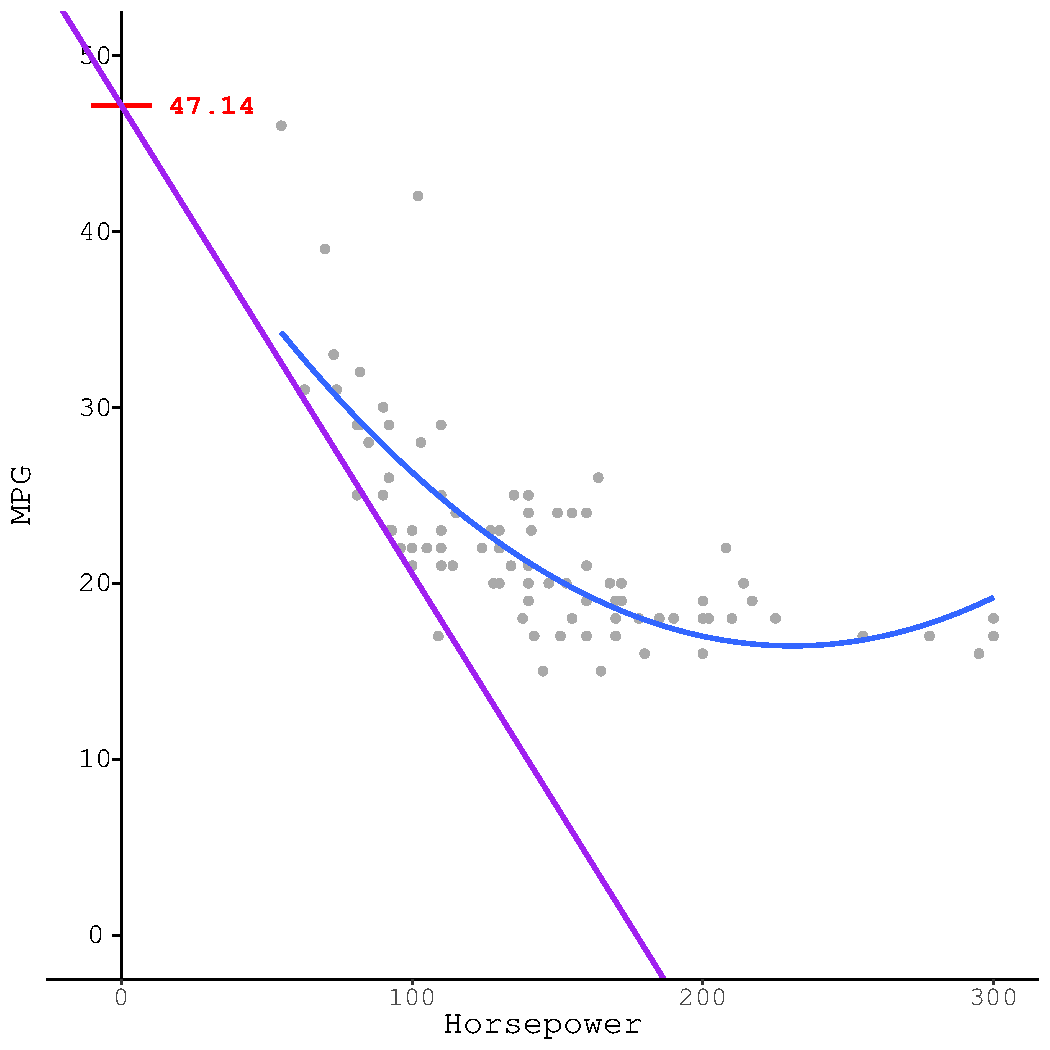
\includegraphics[width=\maxwidth]{figure/unnamed-chunk-35-1} 

}



\end{knitrout}

\end{column}
    
    \begin{column}{0.5\textwidth}
      
\begin{knitrout}\footnotesize
\definecolor{shadecolor}{rgb}{0.878, 0.918, 0.933}\color{fgcolor}

{\centering 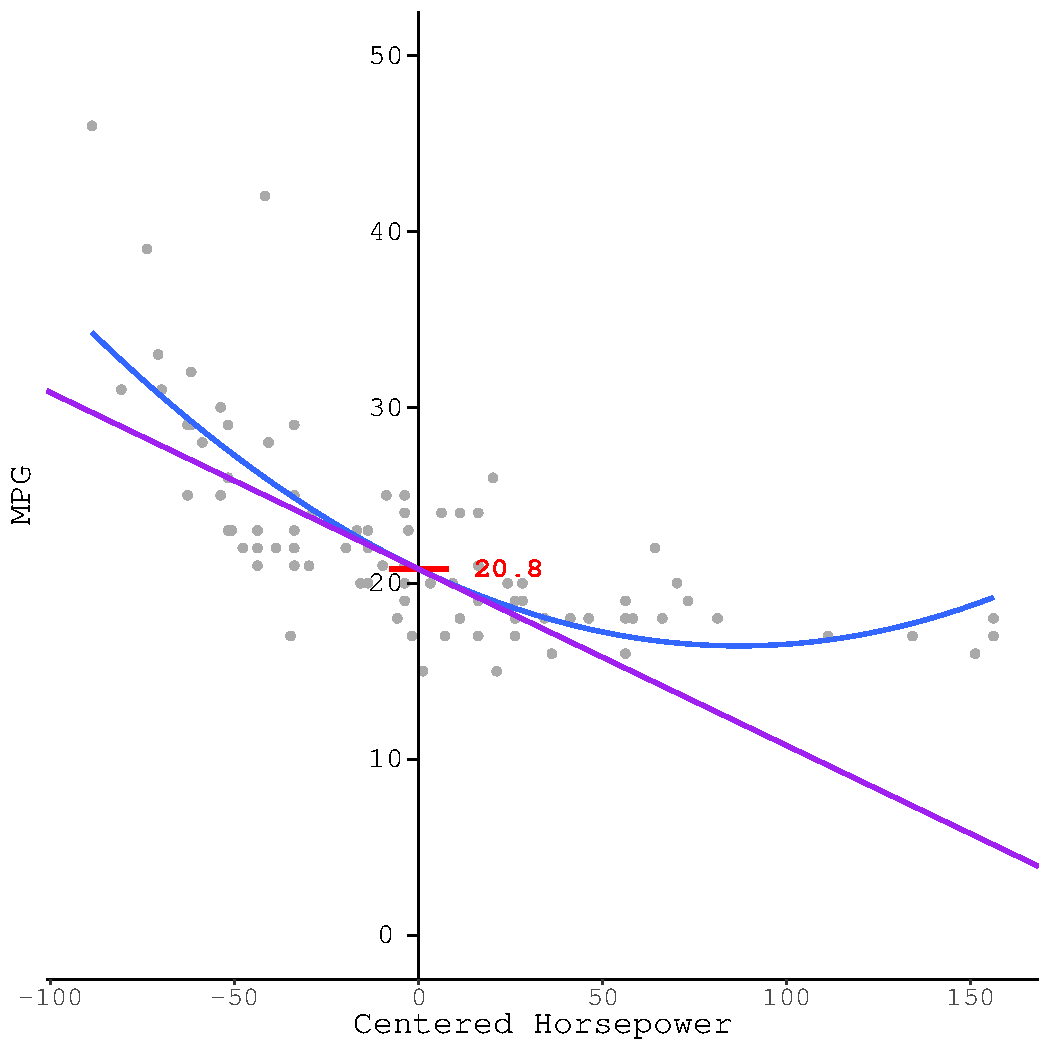
\includegraphics[width=\maxwidth]{figure/unnamed-chunk-36-1} 

}



\end{knitrout}

\end{column}
\end{columns}

\end{frame}

%------------------------------------------------------------------------------%

\begin{frame}[fragile]{Example}

\begin{knitrout}\footnotesize
\definecolor{shadecolor}{rgb}{0.878, 0.918, 0.933}\color{fgcolor}\begin{kframe}
\begin{alltt}
\hlcom{## Mean center horsepower:}
\hlstd{Cars93}\hlopt{$}\hlstd{HorsepowerMC} \hlkwb{<-}
    \hlkwd{with}\hlstd{(Cars93, Horsepower} \hlopt{-} \hlkwd{mean}\hlstd{(Horsepower))}

\hlcom{## Fit the quadratic model:}
\hlstd{out8} \hlkwb{<-} \hlkwd{lm}\hlstd{(MPG.city} \hlopt{~} \hlstd{HorsepowerMC} \hlopt{+} \hlkwd{I}\hlstd{(HorsepowerMC}\hlopt{^}\hlnum{2}\hlstd{),}
           \hlkwc{data} \hlstd{= Cars93)}
\end{alltt}
\end{kframe}
\end{knitrout}

\end{frame}

%------------------------------------------------------------------------------%

\begin{frame}[fragile]{Example}

\begin{knitrout}\footnotesize
\definecolor{shadecolor}{rgb}{0.878, 0.918, 0.933}\color{fgcolor}\begin{kframe}
\begin{alltt}
\hlkwd{partSummary}\hlstd{(out8,} \hlopt{-}\hlkwd{c}\hlstd{(}\hlnum{1}\hlstd{,} \hlnum{2}\hlstd{))}
\end{alltt}
\begin{verbatim}
## Coefficients:
##                     Estimate Std. Error t value Pr(>|t|)
## (Intercept)        2.080e+01  4.422e-01  47.038  < 2e-16
## HorsepowerMC      -1.003e-01  8.320e-03 -12.053  < 2e-16
## I(HorsepowerMC^2)  5.762e-04  9.239e-05   6.237 1.42e-08
## 
## Residual standard error: 3.513 on 90 degrees of freedom
## Multiple R-squared:  0.6177,	Adjusted R-squared:  0.6092 
## F-statistic:  72.7 on 2 and 90 DF,  p-value: < 2.2e-16
\end{verbatim}
\end{kframe}
\end{knitrout}
\vx{-6}
\begin{itemize}
\item Averaging over cars, each unit increase in horsepower, is expected to 
  change fuel economy by $\hat{\beta}_1 = 
  -0.1003$ units.
  \vc
\item For a unit increase in horsepower, the effect of horsepower on fuel 
  economy is expected to increase by $\hat{\beta}_2 = 
  \ensuremath{5.76\times 10^{-4}}$ units.
\end{itemize}

\end{frame}

%------------------------------------------------------------------------------%

\begin{frame}[fragile]{Choosing an ``Optimal'' Polynomial Order}
  
  We can use K-fold cross-validation to estimate which polynomial order will 
  give us the lowest prediction error.
\begin{knitrout}\footnotesize
\definecolor{shadecolor}{rgb}{0.878, 0.918, 0.933}\color{fgcolor}\begin{kframe}
\begin{alltt}
\hlkwd{cv.lm}\hlstd{(}\hlkwc{data}   \hlstd{= Cars93,}
      \hlkwc{models} \hlstd{=} \hlkwd{polyList}\hlstd{(}\hlkwc{y} \hlstd{=} \hlstr{"MPG.city"}\hlstd{,}
                        \hlkwc{x} \hlstd{=} \hlstr{"Horsepower"}\hlstd{,}
                        \hlkwc{n} \hlstd{=} \hlnum{5}\hlstd{),}
      \hlkwc{K}      \hlstd{=} \hlnum{5}\hlstd{,}
      \hlkwc{names}  \hlstd{=} \hlkwd{c}\hlstd{(}\hlstr{"line"}\hlstd{,} \hlstr{"quad"}\hlstd{,} \hlstr{"cube"}\hlstd{,} \hlstr{"quart"}\hlstd{,} \hlstr{"quint"}\hlstd{)}
      \hlstd{)}
\end{alltt}
\begin{verbatim}
##     line     quad     cube    quart    quint 
## 17.68113 12.76947 11.33363 11.85176 12.36846
\end{verbatim}
\end{kframe}
\end{knitrout}

\end{frame}

%------------------------------------------------------------------------------%

\begin{frame}{Visualize the Best Model}
  
  \begin{columns}
    \begin{column}{0.5\textwidth}
      
      The cubic model produced the lowest cross-validation error.
      \vc
      \begin{itemize}
      \item $\hat{Y}_{mpg} = +\hat{\beta}_1 X_{hp} + \hat{\beta}_2 X_{hp}^2 + \hat{\beta}_3 X_{hp}^3$
      \item We should be cautious.
        \vc
        \begin{itemize}
        \item We have very few data.
          \vc
        \item The few cases in the tails are strongly influencing the curve.
        \end{itemize}
      \end{itemize}
      
    \end{column}
    
    \begin{column}{0.5\textwidth}
      
\begin{knitrout}\footnotesize
\definecolor{shadecolor}{rgb}{0.878, 0.918, 0.933}\color{fgcolor}

{\centering 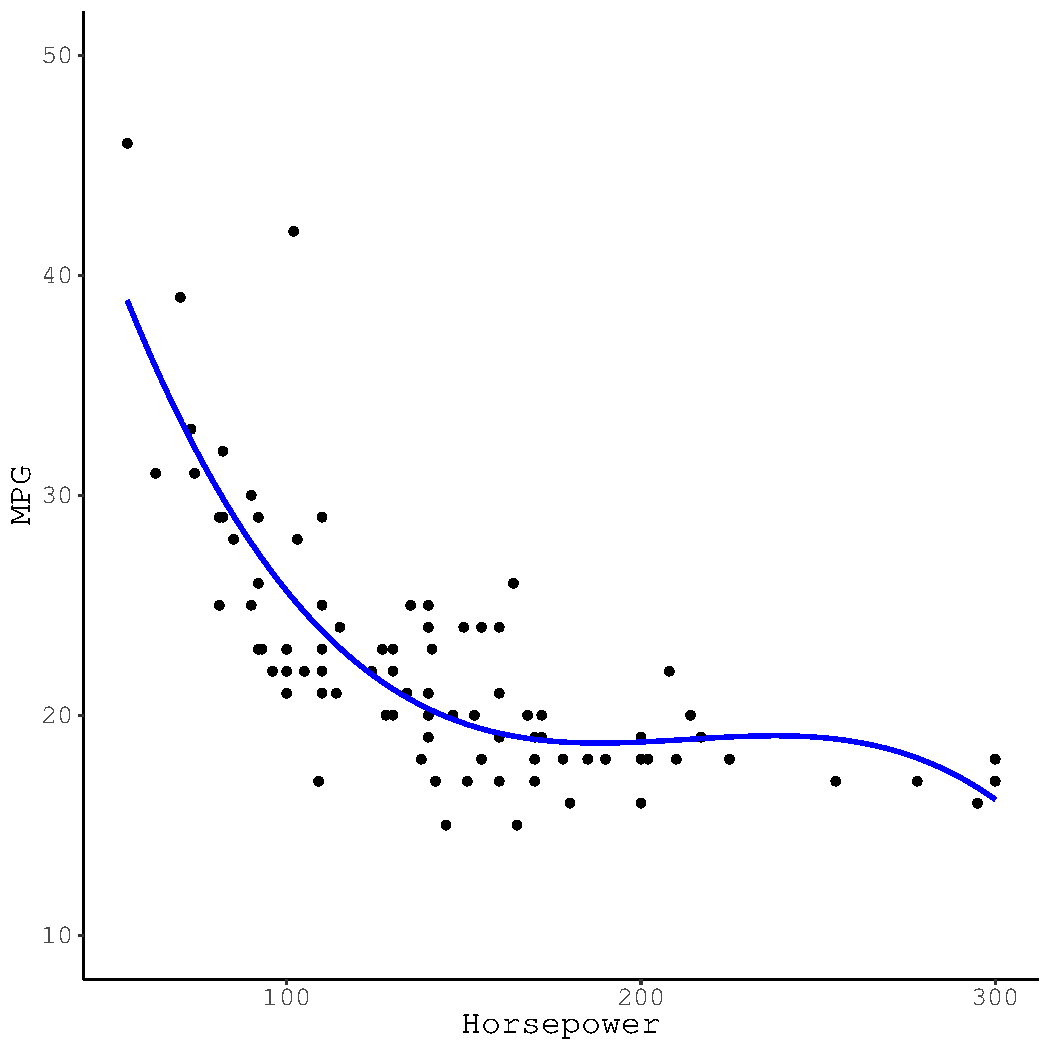
\includegraphics[width=\maxwidth]{figure/unnamed-chunk-40-1} 

}



\end{knitrout}

\end{column}
\end{columns}

\end{frame}

\watermarkon %-----------------------------------------------------------------%

\begin{frame}[allowframebreaks]{Conclusion}
  
  \begin{itemize}
  \item \emph{Moderation} is a specific type of hypothesis.
    \vc
    \begin{itemize}
    \item The effect of one variable on the outcome (i.e., the focal effect) 
      changes as a function of some third variable (i.e., the moderator).
    \end{itemize}
    \vb
  \item We test for significant moderation by modeling \emph{interaction} terms.
    \vc
    \begin{itemize}
    \item If the slope associated with an interaction term is statistically 
      significant, we infer significant moderation.
    \end{itemize}
    \vb
  \item A significant interaction term only tells us that the focal effect is 
    dependent upon the moderator.
    \vc
    \begin{itemize}
    \item We must usually probe significant interactions to get any real insight 
      into the patterns of moderation.
    \end{itemize}
    
    \pagebreak
    
  \item We can probe an interaction by testing specific simple slopes.
    \vc
    \begin{itemize}
    \item \emph{Simple slopes} analysis
    \end{itemize}
    \vb
  \item We can also probe an interaction by finding the region of the 
    moderator's distribution wherein the focal effect is significant.
    \vc
    \begin{itemize}
    \item \emph{Johnson-Neyman} approach
    \end{itemize}
    \vb
  \item Categorical moderators imply group-specific focal effects.
    \vc
    \begin{itemize}
    \item We use simple slopes analysis to probe categorical moderation.
      \vc
    \item Johnson-Neyman doesn't make any sense with discrete moderators.
    \end{itemize}
  
  \pagebreak
  
  \item When we include interactions in our model, the first-order effects of 
    variables involved in the interactions become \emph{conditional effects}.
    \vc
    \begin{itemize}
    \item Conditional effects must be interpreted at the point where the other 
      predictor involved in the interaction is equal to zero.
    \end{itemize}
    \vb
  \item We can use the interpretation of conditional effects to our advantage 
    when testing simple slopes.
    \vc
    \begin{itemize}
    \item Center the moderator on a conditional value and re-run the model.
      \vc
    \item The estimated focal effect is a simple slope.
    \end{itemize}
  
    \pagebreak
    
  \item Polynomial regression models curvilinear trends.
    \vc
    \begin{itemize}
    \item Each unit increase in the order of the polynomial adds another bend to
      the curve.
    \end{itemize}
    \vb
  \item We can think of polynomials as interactions between the focal predictor 
    and itself.
    \vc
    \begin{itemize}
    \item Centering the focal predictors is especially important for 
      interpretation in polynomial regression.
    \end{itemize}
    \vb
  \item We need to be very cautious and constantly watch for overfitting when 
    using polynomial regression.
    \vc
    \begin{itemize}
    \item Even proper cross-validation may not protect us with small samples.
    \end{itemize}
  \end{itemize}
  
\end{frame}
  
%------------------------------------------------------------------------------%

\begin{frame}[allowframebreaks]{References}

  \bibliographystyle{apacite}
  \bibliography{../../../literature/bibtexFiles/statMethRefs.bib}

\end{frame}

\end{document}

